\section{Instance models and instance graphs}
\label{sec:transformation_framework:instance_models_and_instance_graphs}

In the previous section, the structure of the framework was applied to type models and type graphs. In this section, the structure will be applied to instance models and instance graphs. Since instance models and instance graphs directly depend on type models and type graphs, some definitions will be borrowed from the previous section.

First, the general structure of the framework applied to instance models and instance graphs is discussed. Then the required definitions and theorems are given.

\begin{figure}
    \centering
    \begin{tikzpicture} 
    \path
    (-3,4) node[circle,draw,minimum size=10mm,inner sep=0pt](ME) {$O$}
    (-4.5,2) node[circle,draw,minimum size=10mm,inner sep=0pt](MA) {$Im_A$}
    (-1.5,2) node[circle,draw,minimum size=10mm,inner sep=0pt](MB) {$Im_B$}
    (-3,0) node[circle,draw,minimum size=10mm,inner sep=0pt](MAB) {$Im_{AB}$}
    
    (3,4) node[circle,draw,minimum size=10mm,inner sep=0pt](GN) {$N$}
    (1.5,2) node[circle,draw,minimum size=10mm,inner sep=0pt](GA) {$IG_A$}
    (4.5,2) node[circle,draw,minimum size=10mm,inner sep=0pt](GB) {$IG_B$}
    (3,0) node[circle,draw,minimum size=10mm,inner sep=0pt](GAB) {$IG_{AB}$};
    
    \path[]		
    (ME) [-, black, out=240, in=90] edge node[above] {} (MA)
    (ME) [-, black, out=300, in=90] edge node[above] {} (MB)
    
    (MA) [-{Latex[width=5]}, black, out=270, in=90] edge node[above] {} (MAB)
    (MB) [-{Latex[width=5]}, black, out=270, in=90] edge node[above] {} (MAB)
    
    (GN) [-, black, out=240, in=90] edge node[above] {} (GA)
    (GN) [-, black, out=300, in=90] edge node[above] {} (GB)
    
    (GA) [-{Latex[width=5]}, black, out=270, in=90] edge node[above] {} (GAB)
    (GB) [-{Latex[width=5]}, black, out=270, in=90] edge node[above] {} (GAB)
    
    (ME) [-{Latex[width=5]}, black, out=25, in=155] edge node[above] {$f$} (GN)
    (GN) [-{Latex[width=5]}, black, out=165, in=15] edge node[above] {} (ME)
    
    (MA) [-{Latex[width=5]}, black, out=35, in=145] edge node[above] {$f_A$} (GA)
    (GA) [-{Latex[width=5]}, black, out=155, in=25] edge node[above] {} (MA)
    
    (MB) [-{Latex[width=5]}, black, out=35, in=145] edge node[above] {$f_B$} (GB)
    (GB) [-{Latex[width=5]}, black, out=155, in=25] edge node[above] {} (MB)
    
    (MAB) [-{Latex[width=5]}, black, out=25, in=155] edge node[above] {$f_{A} \sqcup f_{B}$} (GAB)
    (GAB) [-{Latex[width=5]}, black, out=165, in=15] edge node[above] {} (MAB)
    ;
    \end{tikzpicture}
    \caption{Structure for transforming between instance models and instance graphs}
    \label{fig:transformation_framework:instance_models_and_instance_graphs:structure_instance_models_graphs}
\end{figure}

\cref{fig:transformation_framework:instance_models_and_instance_graphs:structure_instance_models_graphs} shows one more alternation of the structure proposed in \cref{sec:transformation_framework:structure}. This version of the structure is applied to instance models and instance graphs. As before, instance model $Im_A$ represents the partially build model which corresponds to instance graph $IG_A$ under the transformation function $f_A$. Instance model $Im_B$ represents the next building block to add to this model. It corresponds to instance graph $IG_B$ under the bijective transformation function $f_B$.

Instance models $Im_A$ and $Im_B$ are entirely distinct except for a set objects $O$, which means $O \subseteq Object_{Im_A} \land O \subseteq Object_{Im_B}$. In a similar way, instance graphs $IG_A$ and $IG_B$ are entirely distinct except for a set of nodes $N$, so $N \subseteq N_{IG_A} \land N \subseteq N_{IG_B}$.

Instance models $Im_A$ and $Im_B$ are combined into instance model $Im_{AB}$ using \cref{defin:transformation_framework:instance_models_and_instance_graphs:combining_instance_models:combine}. In a similar way instance graphs $IG_A$ and $IG_B$ are combined into instance graph $IG_{AB}$ using \cref{defin:transformation_framework:instance_models_and_instance_graphs:combining_instance_graphs:combine}. \cref{defin:transformation_framework:instance_models_and_instance_graphs:combining_instance_models:imod_combine_merge_correct} and \cref{defin:transformation_framework:instance_models_and_instance_graphs:combining_instance_graphs:ig_combine_merge_correct} respectively show that $Im_{AB}$ and $IG_{AB}$ are valid. Then \cref{defin:transformation_framework:instance_models_and_instance_graphs:combining_transformation_functions:combination_transformation_function_instance_model_instance_graph} and \cref{defin:transformation_framework:instance_models_and_instance_graphs:combining_transformation_functions:combination_transformation_function_instance_graph_instance_model} can be used to merge the transformation functions $f_A$ and $f_B$ into $f_{A} \sqcup f_{B}$, where \cref{defin:transformation_framework:instance_models_and_instance_graphs:combining_transformation_functions:ig_combine_mapping_correct} and \cref{defin:transformation_framework:instance_models_and_instance_graphs:combining_transformation_functions:ig_combine_mapping_function_correct} show that $f_{A} \sqcup f_{B}$ is again a valid transformation function transforming $Im_{AB}$ to $IG_{AB}$. Similarly, \cref{defin:transformation_framework:instance_models_and_instance_graphs:combining_transformation_functions:imod_combine_mapping_correct} and \cref{defin:transformation_framework:instance_models_and_instance_graphs:combining_transformation_functions:imod_combine_mapping_function_correct} show that the inverse function of $f_{A} \sqcup f_{B}$ is again a valid transformation function transforming $IG_{AB}$ to $Im_{AB}$.

\subsection{Combining instance models}
\label{subsec:transformation_framework:instance_models_and_instance_graphs:combining_instance_models}

The structure of \cref{fig:transformation_framework:instance_models_and_instance_graphs:structure_instance_models_graphs} shows that the instance models $Im_A$ and $Im_B$ are combined into one instance model $Im_{AB}$. This section provides the definition of this combination and its corresponding theorems. Please note that the definitions presented here are as generic as possible, and do not actively take into account that $Im_{A}$ and $Im_{B}$ are mostly distinct. This bit of information is added later as part of a theorem and proof.

\begin{defin}[Combination function on type models]
\label{defin:transformation_framework:instance_models_and_instance_graphs:combining_instance_models:combine}
$\mathrm{combine}$ is a binary function on two instance models which combines two instance models into one instance model. Assume $Im_A$ is an instance model typed by type model $Tm_A$ and $Im_B$ is an instance model typed by type model $Tm_B$, then $\mathrm{combine}(Im_A, Im_B)$ is typed by $\mathrm{combine}(Tm_A, Tm_B)$ and is defined as follows:
\begin{align*}
\mathrm{combine}(Im_A, Im_B) = \langle&
Object = Object_{Im_A} \cup Object_{Im_B} \\&
\mathrm{ObjectClass} = \mathrm{objectclass\_\!combine}(Im_A, Im_B) \\&
\mathrm{ObjectId} = \mathrm{objectid\_\!combine}(Im_A, Im_B) \\&
\mathrm{FieldValue} = \mathrm{fieldvalue\_\!combine}(Im_A, Im_B) \\&
\mathrm{DefaultValue} = \mathrm{defaultvalue\_\!combine}(Im_A, Im_B)\rangle
\end{align*}

In which $\mathrm{objectclass\_\!combine}$ is given as part of \cref{defin:transformation_framework:instance_models_and_instance_graphs:combining_instance_models:objectclass_combine}, $\mathrm{objectid\_\!combine}$ as part of \cref{defin:transformation_framework:instance_models_and_instance_graphs:combining_instance_models:objectid_combine}, $\mathrm{fieldvalue\_\!combine}$ as part of \cref{defin:transformation_framework:instance_models_and_instance_graphs:combining_instance_models:fieldvalue_combine} and $\mathrm{defaultvalue\_\!combine}$ as part of \cref{defin:transformation_framework:instance_models_and_instance_graphs:combining_instance_models:defaultvalue_combine}.
\isabellelref{imod_combine}{Ecore.Instance_Model_Combination}
\end{defin}

The combination of two instance models knows a surprisingly simple definition. This is mostly caused by the fact that an instance model only contains of a set of objects, which has some properties. The properties of each object are specified by the different functions, which will be introduced in the following definitions.

First, the function for the combination of object classes is discussed.

\begin{defin}[Combination function for object classes]
\label{defin:transformation_framework:instance_models_and_instance_graphs:combining_instance_models:objectclass_combine}
$\mathrm{objectclass\_\!combine}$ is a partial function on two instance models which returns a new function \\$Object_{Im_{AB}} \Rightarrow Class_{Tm_{AB}}$. It is defined as follows:
\begin{multline*}
    \mathrm{objectclass\_\!combine}(Im_{A}, Im_{B}, o) = \\
        \begin{cases}
        \mathrm{ObjectClass}_{Im_A}(o) & \mathrm{if }\ o \in Object_{Im_A} \cap Object_{Im_B} \land \mathrm{ObjectClass}_{Im_A}(o) = \mathrm{ObjectClass}_{Im_B}(o) \\
        \mathrm{ObjectClass}_{Im_A}(o) & \mathrm{if }\ o \in Object_{Im_A} \setminus Object_{Im_B} \\
        \mathrm{ObjectClass}_{Im_B}(o) & \mathrm{if }\ o \in Object_{Im_B} \setminus Object_{Im_A}
    \end{cases}
\end{multline*}
\isabellelref{imod_combine_object_class}{Ecore.Instance_Model_Combination}
\end{defin}

The combination of two instance models knows a surprisingly simple definition. Because an instance model is essentially a set of objects with properties, no complex definition is needed. The properties of each object are specified by the different functions, which will be introduced in the following definitions.

First, the function of the combination of object classes is discussed.

\begin{defin}[Combination function for object identifiers]
\label{defin:transformation_framework:instance_models_and_instance_graphs:combining_instance_models:objectid_combine}
$\mathrm{objectid\_\!combine}$ is a partial function on two instance models which returns a new function \\$Object_{Im_{AB}} \Rightarrow Name$. It is defined as follows:
\begin{multline*}
    \mathrm{objectid\_\!combine}(Im_{A}, Im_{B}, o) = \\
        \begin{cases}
        \mathrm{ObjectId}_{Im_A}(o) & \mathrm{if }\ o \in Object_{Im_A} \cap Object_{Im_B} \land \mathrm{ObjectId}_{Im_A}(o) = \mathrm{ObjectId}_{Im_B}(o) \\
        \mathrm{ObjectId}_{Im_A}(o) & \mathrm{if }\ o \in Object_{Im_A} \setminus Object_{Im_B} \\
        \mathrm{ObjectId}_{Im_B}(o) & \mathrm{if }\ o \in Object_{Im_B} \setminus Object_{Im_A}
    \end{cases}
\end{multline*}
\isabellelref{imod_combine_object_id}{Ecore.Instance_Model_Combination}
\end{defin}

As mentioned before, the definition of the combination function of object identifiers is very similar to the definition of the combination function of object classes. If an object only occurs in one of the instance models, its identifier is copied over. If an object appears in both instance models, they must have the same identifier already in order to have an identifier in the final model.

A careful reader might notice that the behaviour of the function is strange. Theoretically, it might give rise to double identities, which is undesired. As will be shown later, the combination function and theorems assume that the identities of the models are already distinct. This assumption is fair, as it is possible to redefine two instance models to have distinct identities, without loss of significance.

The following definition describes the combination of field values.

\begin{defin}[Combination function for field values]
\label{defin:transformation_framework:instance_models_and_instance_graphs:combining_instance_models:fieldvalue_combine}
$\mathrm{fieldvalue\_\!combine}$ is a partial function on two instance models which returns a new function \\$(Object_{Im_{AB}} \times Field_{Tm_{AB}}) \Rightarrow Value_{Im_{AB}}$. It is defined as follows:
\begin{multline*}
    \mathrm{fieldvalue\_\!combine}(Im_A, Im_B, ( o, f )) = \\
    \begin{cases}
        \mathrm{FieldValue}_{Im_A}(( o, f )) & \mathrm{if}\ o \in Object_{Im_A} \cap Object_{Im_B}\ \land\\&\quad f \in \mathrm{fields}_{Tm_A}(\mathrm{ObjectClass}_{Im_A}(o))\ \land\\&\quad f \in \mathrm{fields}_{Tm_B}(\mathrm{ObjectClass}_{Im_B}(o))\ \land\\&\quad \mathrm{FieldValue}_{Im_A}(( o, f )) = \mathrm{FieldValue}_{Im_B}(( o, f )) \\
        \mathrm{FieldValue}_{Im_A}(( o, f )) & \mathrm{if}\ o \in Object_{Im_A} \land f \in \mathrm{fields}_{Tm_A}(\mathrm{ObjectClass}_{Im_A}(o))\ \land\\&\quad (o \not\in Object_{Im_B} \lor f \not\in \mathrm{fields}_{Tm_B}(\mathrm{ObjectClass}_{Im_B}(o))) \\
        \mathrm{FieldValue}_{Im_B}(( o, f )) & \mathrm{if}\ o \in Object_{Im_B} \land f \in \mathrm{fields}_{Tm_B}(\mathrm{ObjectClass}_{Im_B}(o))\ \land\\&\quad (o \not\in Object_{Im_A} \lor f \not\in \mathrm{fields}_{Tm_A}(\mathrm{ObjectClass}_{Im_A}(o)))
    \end{cases}
\end{multline*}
\isabellelref{imod_combine_field_value}{Ecore.Instance_Model_Combination}
\end{defin}

The definition of the combination function of field values is a lot more complicated than the previous ones. The function domain causes this complexity. Not every combination of an object and a field has a value. An object only has values for those fields that are defined for its class or superclasses.

When a value is set on one of the instance models, but not the other, the value is copied. Furthermore, if a combination of object and field is set for both instance models and the value is the same, it is also copied. Please note that equality is used here, instead of equivalence. This property is to support some mathematical properties later on. Since the transformation framework will not allow for shared fields anyhow, this will not impose problems later.

The last function that needs to be defined is the combination function for default values. It is given in the following definition.

\begin{defin}[Combination function for default values]
\label{defin:transformation_framework:instance_models_and_instance_graphs:combining_instance_models:defaultvalue_combine}
$\mathrm{defaultvalue\_\!combine}$ is a partial function on two instance models which returns a new function \\$Constant_{Tm_{AB}} \Rightarrow Value_{Im_{AB}}$. It is defined as follows:
\begin{multline*}
    \mathrm{defaultvalue\_\!combine}(Im_{A}, Im_{B}, c) = \\
    \begin{cases}
        \mathrm{DefaultValue}_{Im_A}(c) & \mathrm{if }\ c \in Constant_{Tm_A} \cap Constant_{Tm_B}\ \land\\&\quad \mathrm{DefaultValue}_{Im_A}(c) = \mathrm{DefaultValue}_{Im_B}(c) \\
        \mathrm{DefaultValue}_{Im_A}(c) & \mathrm{if }\ c \in Constant_{Tm_A} \setminus Constant_{Tm_B} \\
        \mathrm{DefaultValue}_{Im_B}(c) & \mathrm{if }\ c \in Constant_{Tm_B} \setminus Constant_{Tm_A}
    \end{cases}
\end{multline*}
\isabellelref{imod_combine_default_value}{Ecore.Instance_Model_Combination}
\end{defin}

The definition of the combination function of default values is very similar to the combination function of constant types of type models (see \cref{defin:transformation_framework:type_models_and_type_graphs:combining_type_models:consttype_combine}). This function gives values to constants defined on the type model level. When a constant only appears in the type model of one of the instance models, the value can be copied from that instance model. This behaviour is logical since the other instance model cannot have a value set for that constant. If a constant is set for both of the corresponding type models, the value set on the instance models must be the same. If this is the case, the value can be copied over. This behaviour is desired, as the value for a constant should not change after the combination of two instance models.

Like the last definition, equality is used here to compare the values, instead of equivalence. Once more, this has been done to support some mathematical properties later on. Since the transformation framework will not allow for shared constants anyhow, this will not impose problems later.

With all definitions in place, it is possible to provide an example. Let us return to the multi-protocol chat application example introduced in \cref{fig:transformation_framework:type_models_and_type_graphs:combining_type_models:combine_example} of \cref{subsec:transformation_framework:type_models_and_type_graphs:combining_type_models}. An instance model for $Tm_{Chat}$ (\cref{fig:transformation_framework:type_models_and_type_graphs:combining_type_models:combine_example_tmod1}) could have an instance of a $\type{Thread}$ with some $\type{Message}$s. Formally, the instance model could look as follows:

\begin{align*}
Im_{Chat} =\ &\langle&
Object =\ &\{ 1, 2, 3 \} \\&&
\mathrm{ObjectClass} =\ &\{
( 1, \type{.Thread} ),
( 2, \type{.Message} ),
( 3, \type{.Message} )
\} \\&&
\mathrm{ObjectId} =\ &\{
( 1, \text{Thread42} ),
( 2, \text{Message4084} ),
( 3, \text{Message4093} )
\} \\&&
\mathrm{FieldValue} =\ &\Big\{
\Big( \big( 1, ( \type{.Thread}, \type{id} ) \big), \big[ \type{string}, \text{``BLUB-E\_Thread\_01''} \big] \Big),\\&&&
\Big( \big( 1, ( \type{.Thread}, \type{proto} ) \big), \big[ \type{enum}, ( \type{.Protocol}, \type{BLUB\!-\!E} ) \big] \Big),\\&&&
\Big( \big( 1, ( \type{.Thread}, \type{messages} ) \big), \big[ \type{seqof}, \big\langle [ \type{obj}, 2 ], [ \type{obj}, 3 ] \big\rangle \big] \Big),\\&&&
\Big( \big( 2, ( \type{.Message}, \type{text} ) \big), \big[ \type{string}, \text{``This is a test''} \big] \Big),\\&&&
\Big( \big( 3, ( \type{.Message}, \type{text} ) \big), \big[ \type{string}, \text{``Did you receive it?''} \big] \Big)
\Big\} \\&&
\mathrm{DefaultValue} =\ &\{\}
\\&\rangle
\end{align*}

A visual representation of this instance model is included in \cref{fig:transformation_framework:instance_models_and_instance_graphs:combining_instance_models:combine_example_imod1}. Now, assume that there also exists some instance model that is typed by the extension represented by $Tm_{Extension}$. This instance model introduces a $\type{Contact}$ instance for the $\type{Thread}$ instance in $Im_{Chat}$. Formally, this instance model could be defined as follows:

\begin{align*}
Im_{Extension} =\ &\langle&
Object =\ &\{ 1, 4 \} \\&&
\mathrm{ObjectClass} =\ &\{
( 1, \type{.Thread} ),
( 4, \type{.Contact} )
\} \\&&
\mathrm{ObjectId} =\ &\{
( 1, \text{Thread42} ),
( 4, \text{Broodkast} )
\} \\&&
\mathrm{FieldValue} =\ &\Big\{
\Big( \big( 1, ( \type{.Thread}, \type{contact} ) \big), \big[ \type{obj}, 4 \big] \Big),\\&&&
\Big( \big( 4, ( \type{.Contact}, \type{id} ) \big), \big[ \type{data}, \text{``BLUB-E\_PubKey\_a8138''} \big] \Big),\\&&&
\Big( \big( 4, ( \type{.Contact}, \type{name} ) \big), \big[ \type{string}, \text{``Lukas''} \big] \Big)
\Big\} \\&&
\mathrm{DefaultValue} =\ &\{\}
\\&\rangle
\end{align*}

The visual representation of $Im_{Extension}$ is included in \cref{fig:transformation_framework:instance_models_and_instance_graphs:combining_instance_models:combine_example_imod2}. With these instance models formally defined, it is possible to combine them using \cref{defin:transformation_framework:instance_models_and_instance_graphs:combining_instance_models:combine}. This will yield the following model:

\begin{align*}
Im_{ChatExt} =\ &\langle&
Object =\ &\{ 1, 2, 3, 4 \} \\&&
\mathrm{ObjectClass} =\ &\{
( 1, \type{.Thread} ),
( 2, \type{.Message} ),
( 3, \type{.Message} ),
( 4, \type{.Contact} )
\} \\&&
\mathrm{ObjectId} =\ &\{
( 1, \text{Thread42} ),
( 2, \text{Message4084} ),
( 3, \text{Message4093} ),
( 4, \text{Broodkast} )
\} \\&&
\mathrm{FieldValue} =\ &\Big\{
\Big( \big( 1, ( \type{.Thread}, \type{id} ) \big), \big[ \type{string}, \text{``BLUB-E\_Thread\_01''} \big] \Big),\\&&&
\Big( \big( 1, ( \type{.Thread}, \type{proto} ) \big), \big[ \type{enum}, ( \type{.Protocol}, \type{BLUB\!-\!E} ) \big] \Big),\\&&&
\Big( \big( 1, ( \type{.Thread}, \type{messages} ) \big), \big[ \type{seqof}, \big\langle [ \type{obj}, 2 ], [ \type{obj}, 3 ] \big\rangle \big] \Big),\\&&&
\Big( \big( 1, ( \type{.Thread}, \type{contact} ) \big), \big[ \type{obj}, 4 \big] \Big),\\&&&
\Big( \big( 2, ( \type{.Message}, \type{text} ) \big), \big[ \type{string}, \text{``This is a test''} \big] \Big),\\&&&
\Big( \big( 3, ( \type{.Message}, \type{text} ) \big), \big[ \type{string}, \text{``Did you receive it?''} \big] \Big),\\&&&
\Big( \big( 4, ( \type{.Contact}, \type{id} ) \big), \big[ \type{data}, \text{``BLUB-E\_PubKey\_a8138''} \big] \Big),\\&&&
\Big( \big( 4, ( \type{.Contact}, \type{name} ) \big), \big[ \type{string}, \text{``Lukas''} \big] \Big)
\Big\} \\&&
\mathrm{DefaultValue} =\ &\{\}
\\&\rangle
\end{align*}

A visual representation of this combined model is included as \cref{fig:transformation_framework:instance_models_and_instance_graphs:combining_instance_models:combine_example_imod12}. Like the example for the combination of type models, this example shows that the definition of the combination of instance models is useful. It allows to build larger models out of smaller building blocks. Furthermore, the example shows that the combination of the two instance models is typed by the combination of its corresponding type models.

\begin{figure}
    \centering
    \begin{subfigure}{\textwidth}
        \centering
        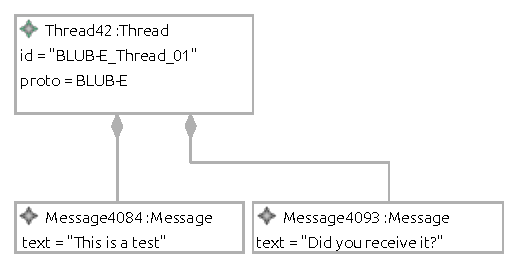
\includegraphics{images/04_transformation_framework/instance_models_combination/chat_instance_partial1.pdf}
        \caption{The chat application instance model $Im_{Chat}$}
        \label{fig:transformation_framework:instance_models_and_instance_graphs:combining_instance_models:combine_example_imod1}
    \end{subfigure}
    \par\medskip
    \begin{subfigure}{\textwidth}
        \centering
        
\includegraphics{images/04_transformation_framework/instance_models_combination/chat_instance_partial2.pdf}
        \caption{The contact extension instance model $Im_{Extension}$}
        \label{fig:transformation_framework:instance_models_and_instance_graphs:combining_instance_models:combine_example_imod2}
    \end{subfigure}
    \par\medskip
    \begin{subfigure}{\textwidth}
        \centering
        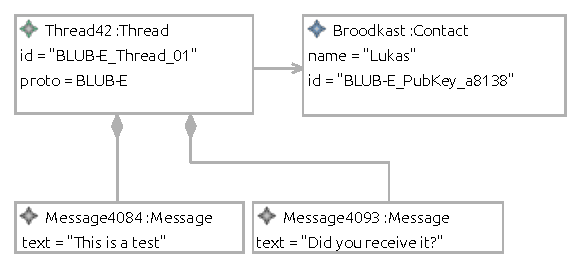
\includegraphics{images/04_transformation_framework/instance_models_combination/chat_instance_combined.pdf}
        \caption{The extended chat application instance model $Im_{ChatExt}$}
        \label{fig:transformation_framework:instance_models_and_instance_graphs:combining_instance_models:combine_example_imod12}
    \end{subfigure}
    \caption{Example of the combination of type models}
    \label{fig:transformation_framework:instance_models_and_instance_graphs:combining_instance_models:combine_example}
\end{figure}

Although the definitions of the combination of instance models are given, no mathematical properties or theorems are defined yet. Some mathematical properties hold for the combination of instance models, that will be presented in the following theorems.

\begin{thm}[Commutativity of the combination of instance models]
\label{defin:transformation_framework:instance_models_and_instance_graphs:combining_instance_models:imod_combine_commute}
Assume that $Im_A$ and $Im_B$ are instance models, then the $\mathrm{combine}$ function is commutative:
\begin{equation*}
    \mathrm{combine}(Im_A, Im_B) = \mathrm{combine}(Im_B, Im_A)
\end{equation*}
\isabellelref{imod_combine_commute}{Ecore.Instance_Model_Combination}
\end{thm}

\begin{thm}[Associativity of the combination of instance models]
\label{defin:transformation_framework:instance_models_and_instance_graphs:combining_instance_models:imod_combine_assoc}
Assume that $Im_A$, $Im_B$ and $Im_C$ are instance models, then the $\mathrm{combine}$ function is associative:
\begin{equation*}
    \mathrm{combine}(\mathrm{combine}(Im_A, Im_B), Im_C) = \mathrm{combine}(Im_A, \mathrm{combine}(Im_B, Im_C))
\end{equation*}
\isabellelref{imod_combine_assoc}{Ecore.Instance_Model_Combination}
\end{thm}

\begin{thm}[Idempotence of the combination of instance models]
\label{defin:transformation_framework:instance_models_and_instance_graphs:combining_instance_models:imod_combine_idemp}
Assume that $Im_A$ is an instance model and that it is valid in the sense of \cref{defin:formalisations:ecore_formalisation:instance_models:model_validity}. Then the following property holds:
\begin{equation*}
    \mathrm{combine}(Im_A, Im_A) = Im_A
\end{equation*}
\isabellelref{imod_combine_idemp_alt}{Ecore.Instance_Model_Combination}
\end{thm}

These properties follow directly from \cref{defin:transformation_framework:instance_models_and_instance_graphs:combining_instance_models:combine}, but the corresponding proofs will not be included here. It should be noted that these properties are indeed proven correct as part of this thesis, and the corresponding proofs are validated within Isabelle.

Besides these properties, the combination of instance models also has an identity element. The empty instance model represents this identity element, but it needs to be defined first:

\begin{defin}[Empty instance model]
\label{defin:transformation_framework:instance_models_and_instance_graphs:combining_instance_models:empty_instance_model}
Let $Im_{\epsilon}$ be the empty instance model. It is typed by the empty type model $Tm_{\epsilon}$. $Im_{\epsilon}$ is defined as:
\begin{align*}
Im_{\epsilon} = \langle&
Object = \{\} \\&
\mathrm{ObjectClass} = undefined \\&
\mathrm{ObjectId} = undefined \\&
\mathrm{FieldValue} = undefined \\&
\mathrm{DefaultValue} = undefined\rangle
\end{align*}
\end{defin}

\begin{thm}[Correctness of the empty type model]
\label{defin:transformation_framework:instance_models_and_instance_graphs:combining_instance_models:imod_empty_correct}
The empty instance model, $Im_{\epsilon}$, is valid with respect to
\cref{defin:formalisations:ecore_formalisation:instance_models:model_validity}.
\isabellelref{imod_empty_correct}{Ecore.Instance_Model}
\end{thm}

The proof for the correctness of the empty instance model is trivial. Still, a validated version of this proof can be found within the Isabelle theories of this thesis.

As mentioned earlier, the empty instance model acts as an identity element when combining two instance models. The following theorem specifies this behaviour.

\begin{thm}[Identity of the combination of instance models]
\label{defin:transformation_framework:instance_models_and_instance_graphs:combining_instance_models:imod_combine_identity}
Assume that $Im_A$ is an instance model and that it is valid in the sense of \cref{defin:formalisations:ecore_formalisation:instance_models:model_validity}. Then $Im_{\epsilon}$ acts as an identity element in the combination function:
\begin{equation*}
    \mathrm{combine}(Im_{\epsilon}, Im_A) = Im_A
\end{equation*}
\isabellelref{imod_combine_identity_alt}{Ecore.Instance_Model_Combination}
\end{thm}

Once more, the proof of this theorem follows directly from the definition. Therefore, the corresponding proof will not be included here, but a validated version can be found within the Isabelle theories of this thesis.

A final desired property for the combination of instance models is a correctness property. \cref{defin:transformation_framework:instance_models_and_instance_graphs:combining_instance_models:imod_combine_correct} defines the theorem under which the combination of instance models is a valid instance model. Please note that this theorem is a generic theorem, which does not take into account that the instance models are mostly distinct.

\begin{thm}[Validity of the combination of instance models]
\label{defin:transformation_framework:instance_models_and_instance_graphs:combining_instance_models:imod_combine_correct}
Assume that $Im_A$ and $Im_B$ are valid instance models in the sense of \cref{defin:formalisations:ecore_formalisation:instance_models:model_validity}. Assume that $Im_A$ is typed by type model $Tm_A$. Furthermore, assume that $Im_B$ is typed by type model $Tm_B$. $Tm_A$ and $Tm_B$ are consistent by definition. Also assume that $Tm_{AB} = \mathrm{combine}(Tm_A, Tm_B)$ is consistent in the sense of \cref{defin:formalisations:ecore_formalisation:type_models:type_model_consistency}. Finally, assume the following properties:
\begin{itemize}
    \item For all shared objects, the object class must be the same in both instance models: $\forall o \in Object_{Im_A} \cap Object_{Im_B}\!: \mathrm{ObjectClass}_{Im_A}(o) = \mathrm{ObjectClass}_{Im_B}(o)$.
    \item For all shared objects, the object id must be the same in both instance models: $\forall o \in Object_{Im_A} \cap Object_{Im_B}\!: \mathrm{ObjectId}_{Im_A}(o) = \mathrm{ObjectId}_{Im_B}(o)$.
    \item For all shared constants within the corresponding type graphs, the default value must be the same in both instance models: $\forall c \in Constant_{Tm_A} \cap Constant_{Tm_B}\!:$\\$\mathrm{DefaultValue}_{Im_A}(c) = \mathrm{DefaultValue}_{Im_B}(c)$.
    \item The identifiers must be unique across both instance models: $\forall o_1 \in Object_{Im_A} \setminus Object_{Im_B} \land o_2 \in Object_{Im_B} \setminus Object_{Im_A}\!: \mathrm{ObjectId}_{Im_A}(o_1) = \mathrm{ObjectId}_{Im_B}(o_2) \implies o_1 = o_2$.
    \item If a field value is set for a combination of an object and field in both instance models, that field value must be the same in both instance models: $\forall o \in Object_{Im_A} \cap Object_{Im_B}\ \land$\\$f \in \mathrm{fields}_{Tm_A}(\mathrm{ObjectClass}_{Im_A}(o)) \cap \mathrm{fields}_{Tm_B}(\mathrm{ObjectClass}_{Im_B}(o))\!:$\\$\mathrm{FieldValue}_{Im_A}(( o, f )) = \mathrm{FieldValue}_{Im_B}(( o, f ))$.
    \item If an object needs a field value in the combination of $Im_A$ and $Im_B$, but this field value is not set in $Im_A$, then it must be set in $Im_B$:
    $\forall o \in Object_{Im_A} \land f \not\in \mathrm{fields}_{Tm_A}(\mathrm{ObjectClass}_{Im_A}(o))\!:
    f \in \mathrm{fields}_{Tm_{AB}}(\mathrm{ObjectClass}_{\mathrm{combine}(Im_A, Im_B)}(o)) \implies$\\$
    o \in Object_{Im_B} \land f \in \mathrm{fields}_{Tm_B}(\mathrm{ObjectClass}_{Im_B}(o))$.
    \item If an object needs a field value in the combination of $Im_A$ and $Im_B$, but this field value is not set in $Im_B$, then it must be set in $Im_A$:
    $\forall o \in Object_{Im_B} \land f \not\in \mathrm{fields}_{Tm_B}(\mathrm{ObjectClass}_{Im_B}(o))\!:
    f \in \mathrm{fields}_{Tm_{AB}}(\mathrm{ObjectClass}_{\mathrm{combine}(Im_A, Im_B)}(o)) \implies$\\$
    o \in Object_{Im_A} \land f \in \mathrm{fields}_{Tm_A}(\mathrm{ObjectClass}_{Im_A}(o))$.
    \item For field values copied from $Im_A$ that are in $ContainerValue_{Im_A}$, the combined multiplicity must be correct: $\forall o \in Object_{Im_A}\ \land f \in \mathrm{fields}_{Tm_A}(\mathrm{ObjectClass}_{Im_A}(o))\ \land$\\$f \in Field_{Tm_B}\!: \mathrm{FieldValue}_{Im_A}(( o, f )) \in ContainerValue_{Im_A} \implies$\\$\mathrm{lower}_{Tm_{AB}}(\mathrm{FieldSig}_{Tm_{AB}}(f)) \leq |\mathrm{FieldValue}_{Im_A}(( o, f ))|\ \land$\\$|\mathrm{FieldValue}_{Im_A}(( o, f ))| \leq \mathrm{upper}_{Tm_{AB}}(\mathrm{FieldSig}_{Tm_{AB}}(f))$.
    \item For field values copied from $Im_B$ that are in $ContainerValue_{Im_B}$, the combined multiplicity must be correct: $\forall o \in Object_{Im_B}\ \land f \in \mathrm{fields}_{Tm_B}(\mathrm{ObjectClass}_{Im_B}(o))\ \land$\\$f \in Field_{Tm_A}\!: \mathrm{FieldValue}_{Im_B}(( o, f )) \in ContainerValue_{Im_B} \implies$\\$\mathrm{lower}_{Tm_{AB}}(\mathrm{FieldSig}_{Tm_{AB}}(f)) \leq |\mathrm{FieldValue}_{Im_B}(( o, f ))|\ \land$\\$|\mathrm{FieldValue}_{Im_B}(( o, f ))| \leq \mathrm{upper}_{Tm_{AB}}(\mathrm{FieldSig}_{Tm_{AB}}(f))$.
    \item If there exists a containment property in $Tm_{AB}$, the satisfaction formula for containment properties must be satisfied: $\forall o \in Object_{Im_A} \cup Object_{Im_B}\!:$\\$\big|\big\{ \big( ( f\!o, f\!\!f ), f\!v \big) \mid \big( ( f\!o, f\!\!f ), fv \big) \in \mathrm{FieldValue}_{\mathrm{combine}(Im_A, Im_B)} \land [ \type{obj}, o ] = f\!v \land f\!\!f \in CR_{Tm_{AB}} \big\}\big| \leq 1$
    \item There may be no cycles in the containment edges of the combined instance model: $\big\{ (f\!o, f\!v) \mid \big( ( f\!o, f\!\!f ), f\!v \big) \in \mathrm{FieldValue}_{\mathrm{combine}(Im_A, Im_B)} \land f\!\!f \in CR_{Tm_{AB}} \big\}$ is acyclic.
    \item The identity properties must remain satisfied when combining objects from different instance models: $\forall [ \type{identity}, c, A ] \in Prop_{Tm_{A}} \land [ \type{identity}, c, A ] \in Prop_{Tm_{B}} \land o_1 \in Object_{Im_A} \setminus Object_{Im_B} \land o_2 \in Object_{Im_B} \setminus Object_{Im_A} \land \mathrm{ObjectClass}_{Im_A}(o_1) = c \land \mathrm{ObjectClass}_{Im_B}(o_2) = c \land a \in A\!: \mathrm{FieldValue}_{Im_A}(( o_1, a )) \equiv_{\mathrm{combine}(Im_A, Im_B)} \mathrm{FieldValue}_{Im_B}(( o_2, a )) \implies o_1 = o_2$.
    \item The opposite properties must remain satisfied when combining objects from different instance models: $\forall [ \type{opposite}, r_1, r_2 ] \in Prop_{Tm_{A}} \land [ \type{opposite}, r_1, r_2 ] \in Prop_{Tm_{B}}\ \land$\\$o_1 \in Object_{Im_A} \land (o_1 \not\in Object_{Im_B} \lor r_1 \not\in \mathrm{fields}_{Tm_B}(\mathrm{ObjectClass}_{Im_B}(o_1)))\ \land$\\$o_2 \in Object_{Im_B} \land (o_2 \not\in Object_{Im_A} \lor r_2 \not\in \mathrm{fields}_{Tm_A}(\mathrm{ObjectClass}_{Im_A}(o_2))) \implies$\\$ \mathrm{edgeCount}_{Im_A}(o_1, r_1, o_2) = \mathrm{edgeCount}_{Im_B}(o_2, r_2, o_1)$.
\end{itemize}

Then $\mathrm{combine}(Im_A, Im_B)$ is a valid instance model in the sense of \cref{defin:formalisations:ecore_formalisation:instance_models:model_validity}
\isabellelref{imod_combine_correct}{Ecore.Instance_Model_Combination}
\end{thm}

\begin{proof}
To proof that $\mathrm{combine}(Im_A, Im_B)$ is a valid instance model, it needs to be shown that\\ $\mathrm{combine}(Im_A, Im_B)$ gives rise to a valid structure for an instance model and that \cref{defin:formalisations:ecore_formalisation:instance_models:model_validity} holds. For readability, define $Im_{AB}$ to be $\mathrm{combine}(Im_A, Im_B)$.

\emph{Structural properties}
\begin{itemize}
    \item For each object $o$, $\mathrm{ObjectClass}_{Im_{AB}}(o)$ must be an element of $Class_{Tm_{AB}}$.

    If $o \in Object_{Im_A} \setminus Object_{Im_B}$, then $\mathrm{ObjectClass}_{Im_{AB}}(o) \in Class_{Tm_{AB}}$.
    
    Similarly, if $o \in Object_{Im_B} \setminus Object_{Im_A}$, then $\mathrm{ObjectClass}_{Im_{AB}}(o) \in Class_{Tm_{AB}}$.
    
    If $o \in Object_{Im_A} \cap Object_{Im_B}$, then $\mathrm{ObjectClass}_{Im_{A}}(o) = \mathrm{ObjectClass}_{Im_{B}}(o)$ by assumption. Therefore $\mathrm{ObjectClass}_{Im_{AB}}(o) \in Class_{Tm_{AB}}$.


    \item For each object $o$, $\mathrm{ObjectId}_{Im_{AB}}(o)$ must be an element of $Name$.
    
    If $o \in Object_{Im_A} \setminus Object_{Im_B}$, then $\mathrm{ObjectId}_{Im_{AB}}(o) \in Name$.
    
    Similarly, if $o \in Object_{Im_B} \setminus Object_{Im_A}$, then $\mathrm{ObjectId}_{Im_{AB}}(o) \in Name$.
    
    If $o \in Object_{Im_A} \cap Object_{Im_B}$, then $\mathrm{ObjectId}_{Im_{A}}(o) = \mathrm{ObjectId}_{Im_{B}}(o)$ by assumption. Therefore $\mathrm{ObjectId}_{Im_{AB}}(o) \in Name$.
    
    
    \item For each object $o$, and $f \in \mathrm{fields}_{Tm_{AB}}(\mathrm{ObjectClass}_{Im_{AB}}(o))$, $\mathrm{FieldValue}_{Im_{AB}}(( o, f ))$ must be an element of $Value_{Im_{AB}}$.
    
    First, note that $Value_{Im_A} \cup Value_{Im_B} \subseteq Value_{Im_{AB}}$\\(see \isabelleref{imod_combine_value}{Ecore.Instance_Model_Combination}).
    
    If $o \in Object_{Im_A} \setminus Object_{Im_B}$, then $f \in \mathrm{fields}_{Tm_{A}}(\mathrm{ObjectClass}_{Im_{A}}(o))$ or \\$f \not\in \mathrm{fields}_{Tm_{A}}(\mathrm{ObjectClass}_{Im_{A}}(o))$.
    
    \begin{itemize}
        \item If $f \in \mathrm{fields}_{Tm_{A}}(\mathrm{ObjectClass}_{Im_{A}}(o))$, then $\mathrm{FieldValue}_{Im_{AB}}(( o, f )) = \mathrm{FieldValue}_{Im_{A}}(( o, f ))$ and, therefore, $\mathrm{FieldValue}_{Im_{AB}}(( o, f )) \in Value_{Im_{AB}}$.
        
        \item If $f \not\in \mathrm{fields}_{Tm_{A}}(\mathrm{ObjectClass}_{Im_{A}}(o))$, then by assumption, $f \in Object_{Im_B}$. However, $f \not\in Object_{Im_B}$, so this case is invalid.
    \end{itemize}
    
    If $o \in Object_{Im_B} \setminus Object_{Im_A}$, then $f \in \mathrm{fields}_{Tm_{B}}(\mathrm{ObjectClass}_{Im_{B}}(o))$ or \\$f \not\in \mathrm{fields}_{Tm_{B}}(\mathrm{ObjectClass}_{Im_{B}}(o))$.
    
    \begin{itemize}
        \item If $f \in \mathrm{fields}_{Tm_{B}}(\mathrm{ObjectClass}_{Im_{B}}(o))$, then $\mathrm{FieldValue}_{Im_{AB}}(( o, f )) = \mathrm{FieldValue}_{Im_{B}}(( o, f ))$ and, therefore, $\mathrm{FieldValue}_{Im_{AB}}(( o, f )) \in Value_{Im_{AB}}$.
        
        \item If $f \not\in \mathrm{fields}_{Tm_{B}}(\mathrm{ObjectClass}_{Im_{B}}(o))$, then by assumption, $f \in Object_{Im_A}$. However, $f \not\in Object_{Im_A}$, so this case is invalid.
    \end{itemize}
    
    If $o \in Object_{Im_A} \cap Object_{Im_B}$, then \\$f \in \mathrm{fields}_{Tm_{A}}(\mathrm{ObjectClass}_{Im_{A}}(o)) \cap \mathrm{fields}_{Tm_{B}}(\mathrm{ObjectClass}_{Im_{B}}(o))$ or \\$f \not\in \mathrm{fields}_{Tm_{A}}(\mathrm{ObjectClass}_{Im_{A}}(o))$ or $f \not\in \mathrm{fields}_{Tm_{B}}(\mathrm{ObjectClass}_{Im_{B}}(o))$.
    
    \begin{itemize}
        \item If $f \in \mathrm{fields}_{Tm_{A}}(\mathrm{ObjectClass}_{Im_{A}}(o)) \cap \mathrm{fields}_{Tm_{B}}(\mathrm{ObjectClass}_{Im_{B}}(o))$, then \\$\mathrm{FieldValue}_{Im_{AB}}(( o, f )) = \mathrm{FieldValue}_{Im_{A}}(( o, f ))$ and, therefore, \\$\mathrm{FieldValue}_{Im_{AB}}(( o, f )) \in Value_{Im_{AB}}$.
        
        \item If $f \not\in \mathrm{fields}_{Tm_{A}}(\mathrm{ObjectClass}_{Im_{A}}(o))$, then by assumption, $f \in \mathrm{fields}_{Tm_{B}}(\mathrm{ObjectClass}_{Im_{B}}(o))$. Therefore, $\mathrm{FieldValue}_{Im_{AB}}(( o, f )) = \mathrm{FieldValue}_{Im_{B}}(( o, f ))$ which means that \\$\mathrm{FieldValue}_{Im_{AB}}(( o, f )) \in Value_{Im_{AB}}$.
        
        \item If $f \not\in \mathrm{fields}_{Tm_{B}}(\mathrm{ObjectClass}_{Im_{B}}(o))$, then by assumption, $f \in \mathrm{fields}_{Tm_{A}}(\mathrm{ObjectClass}_{Im_{A}}(o))$. Therefore, $\mathrm{FieldValue}_{Im_{AB}}(( o, f )) = \mathrm{FieldValue}_{Im_{A}}(( o, f ))$ which means that \\$\mathrm{FieldValue}_{Im_{AB}}(( o, f )) \in Value_{Im_{AB}}$.
    \end{itemize}
    
    
    \item For each constant $c$ in $Constant_{Tm_{AB}}$, $\mathrm{DefaultValue}_{Im_{AB}}(c)$ must be an element of $Value_{Im_{AB}}$.
    
    First, note that $Value_{Im_A} \cup Value_{Im_B} \subseteq Value_{Im_{AB}}$\\(see \isabelleref{imod_combine_value}{Ecore.Instance_Model_Combination}).
    
    If $c \in Constant_{Tm_A} \setminus Constant_{Tm_B}$, then $\mathrm{DefaultValue}_{Im_{AB}}(c) \in Value_{Im_{AB}}$.
    
    Similarly, if $c \in Constant_{Tm_B} \setminus Constant_{Tm_A}$, then $\mathrm{DefaultValue}_{Im_{AB}}(c) \in Value_{Im_{AB}}$.
    
    If $c \in Constant_{Tm_A} \cap Constant_{Tm_B}$, then $\mathrm{DefaultValue}_{Im_{A}}(c) = \mathrm{DefaultValue}_{Im_{B}}(c)$ by assumption. Therefore $\mathrm{DefaultValue}_{Im_{AB}}(c) \in Value_{Im_{AB}}$.
\end{itemize}

\emph{Validity properties}
\begin{itemize}
    \item $\forall (( o, f ), v ) \in \mathrm{FieldValue}_{Im_{AB}}\!: v:_{Im} \mathrm{type}_{Tm_{AB}}(f)$
    
    If $o \in Object_{Im_A} \setminus Object_{Im_B}$, then $f \in \mathrm{fields}_{Tm_{A}}(\mathrm{ObjectClass}_{Im_{A}}(o))$ or \\$f \not\in \mathrm{fields}_{Tm_{A}}(\mathrm{ObjectClass}_{Im_{A}}(o))$.
    
    \begin{itemize}
        \item If $f \in \mathrm{fields}_{Tm_{A}}(\mathrm{ObjectClass}_{Im_{A}}(o))$, then $\mathrm{FieldValue}_{Im_{AB}}(( o, f )) = \mathrm{FieldValue}_{Im_{A}}(( o, f ))$. In this case $\mathrm{type}_{Tm_{AB}}(f) = \mathrm{type}_{Tm_{A}}(f)$ because types are preserved by $Tm_{AB}$. Therefore, $v:_{Im} \mathrm{type}_{Tm_{AB}}(f)$.
        
        \item If $f \not\in \mathrm{fields}_{Tm_{A}}(\mathrm{ObjectClass}_{Im_{A}}(o))$, then by assumption, $f \in Object_{Im_B}$. However, $f \not\in Object_{Im_B}$, so this case is invalid.
    \end{itemize}
    
    If $o \in Object_{Im_B} \setminus Object_{Im_A}$, then $f \in \mathrm{fields}_{Tm_{B}}(\mathrm{ObjectClass}_{Im_{B}}(o))$ or \\$f \not\in \mathrm{fields}_{Tm_{B}}(\mathrm{ObjectClass}_{Im_{B}}(o))$.
    
    \begin{itemize}
        \item If $f \in \mathrm{fields}_{Tm_{B}}(\mathrm{ObjectClass}_{Im_{B}}(o))$, then $\mathrm{FieldValue}_{Im_{AB}}(( o, f )) = \mathrm{FieldValue}_{Im_{B}}(( o, f ))$. In this case $\mathrm{type}_{Tm_{AB}}(f) = \mathrm{type}_{Tm_{B}}(f)$ because types are preserved by $Tm_{AB}$. Therefore, $v:_{Im} \mathrm{type}_{Tm_{AB}}(f)$.
        
        \item If $f \not\in \mathrm{fields}_{Tm_{B}}(\mathrm{ObjectClass}_{Im_{B}}(o))$, then by assumption, $f \in Object_{Im_A}$. However, $f \not\in Object_{Im_A}$, so this case is invalid.
    \end{itemize}
    
    If $o \in Object_{Im_A} \cap Object_{Im_B}$, then \\$f \in \mathrm{fields}_{Tm_{A}}(\mathrm{ObjectClass}_{Im_{A}}(o)) \cap \mathrm{fields}_{Tm_{B}}(\mathrm{ObjectClass}_{Im_{B}}(o))$ or \\$f \not\in \mathrm{fields}_{Tm_{A}}(\mathrm{ObjectClass}_{Im_{A}}(o))$ or $f \not\in \mathrm{fields}_{Tm_{B}}(\mathrm{ObjectClass}_{Im_{B}}(o))$.
    
    \begin{itemize}
        \item If $f \in \mathrm{fields}_{Tm_{A}}(\mathrm{ObjectClass}_{Im_{A}}(o)) \cap \mathrm{fields}_{Tm_{B}}(\mathrm{ObjectClass}_{Im_{B}}(o))$, then \\$\mathrm{FieldValue}_{Im_{AB}}(( o, f )) = \mathrm{FieldValue}_{Im_{A}}(( o, f ))$. In this case $\mathrm{type}_{Tm_{AB}}(f) = \mathrm{type}_{Tm_{A}}(f)$ because types are preserved by $Tm_{AB}$. Therefore, $v:_{Im} \mathrm{type}_{Tm_{AB}}(f)$.
        
        \item If $f \not\in \mathrm{fields}_{Tm_{A}}(\mathrm{ObjectClass}_{Im_{A}}(o))$, then by assumption, $f \in \mathrm{fields}_{Tm_{B}}(\mathrm{ObjectClass}_{Im_{B}}(o))$. Therefore, $\mathrm{FieldValue}_{Im_{AB}}(( o, f )) = \mathrm{FieldValue}_{Im_{B}}(( o, f ))$. Furthermore, $\mathrm{type}_{Tm_{AB}}(f) = \mathrm{type}_{Tm_{A}}(f)$ because types are preserved by $Tm_{AB}$. Therefore, $v:_{Im} \mathrm{type}_{Tm_{AB}}(f)$.
        
        \item If $f \not\in \mathrm{fields}_{Tm_{B}}(\mathrm{ObjectClass}_{Im_{B}}(o))$, then by assumption, $f \in \mathrm{fields}_{Tm_{A}}(\mathrm{ObjectClass}_{Im_{A}}(o))$. Therefore, $\mathrm{FieldValue}_{Im_{AB}}(( o, f )) = \mathrm{FieldValue}_{Im_{A}}(( o, f ))$. Furthermore, $\mathrm{type}_{Tm_{AB}}(f) = \mathrm{type}_{Tm_{A}}(f)$ because types are preserved by $Tm_{AB}$. Therefore, $v:_{Im} \mathrm{type}_{Tm_{AB}}(f)$.
    \end{itemize}
    
    
    \item $\forall (( o, f ), v ) \in \mathrm{FieldValue}_{Im_{AB}}\!: \mathrm{validMul}_{Im_{AB}}(v)$.
    
    If $o \in Object_{Im_A} \setminus Object_{Im_B}$, then $f \in \mathrm{fields}_{Tm_{A}}(\mathrm{ObjectClass}_{Im_{A}}(o))$ or \\$f \not\in \mathrm{fields}_{Tm_{A}}(\mathrm{ObjectClass}_{Im_{A}}(o))$.
    
    \begin{itemize}
        \item If $f \in \mathrm{fields}_{Tm_{A}}(\mathrm{ObjectClass}_{Im_{A}}(o))$, then $\mathrm{FieldValue}_{Im_{AB}}(( o, f )) = \mathrm{FieldValue}_{Im_{A}}(( o, f ))$. Because $Im_{A}$ is valid, $\mathrm{validMul}_{Im_{A}}(v)$ holds. If the multiplicity is preserved because $f \not\in Field_{Tm_B}$, then $\mathrm{validMul}_{Im_{AB}}(v)$. If the multiplicity is changed because $f \in Field_{Tm_B}$, then $\mathrm{validMul}_{Im_{AB}}(v)$ is proven by assumption.
        
        \item If $f \not\in \mathrm{fields}_{Tm_{A}}(\mathrm{ObjectClass}_{Im_{A}}(o))$, then by assumption, $f \in Object_{Im_B}$. However, $f \not\in Object_{Im_B}$, so this case is invalid.
    \end{itemize}
    
    If $o \in Object_{Im_B} \setminus Object_{Im_A}$, then $f \in \mathrm{fields}_{Tm_{B}}(\mathrm{ObjectClass}_{Im_{B}}(o))$ or \\$f \not\in \mathrm{fields}_{Tm_{B}}(\mathrm{ObjectClass}_{Im_{B}}(o))$.
    
    \begin{itemize}
        \item If $f \in \mathrm{fields}_{Tm_{B}}(\mathrm{ObjectClass}_{Im_{B}}(o))$, then $\mathrm{FieldValue}_{Im_{AB}}(( o, f )) = \mathrm{FieldValue}_{Im_{B}}(( o, f ))$. Because $Im_{B}$ is valid, $\mathrm{validMul}_{Im_{B}}(v)$ holds. If the multiplicity is preserved because $f \not\in Field_{Tm_A}$, then $\mathrm{validMul}_{Im_{AB}}(v)$. If the multiplicity is changed because $f \in Field_{Tm_A}$, then $\mathrm{validMul}_{Im_{AB}}(v)$ is proven by assumption.
        
        \item If $f \not\in \mathrm{fields}_{Tm_{B}}(\mathrm{ObjectClass}_{Im_{B}}(o))$, then by assumption, $f \in Object_{Im_A}$. However, $f \not\in Object_{Im_A}$, so this case is invalid.
    \end{itemize}
    
    If $o \in Object_{Im_A} \cap Object_{Im_B}$, then \\$f \in \mathrm{fields}_{Tm_{A}}(\mathrm{ObjectClass}_{Im_{A}}(o)) \cap \mathrm{fields}_{Tm_{B}}(\mathrm{ObjectClass}_{Im_{B}}(o))$ or \\$f \not\in \mathrm{fields}_{Tm_{A}}(\mathrm{ObjectClass}_{Im_{A}}(o))$ or $f \not\in \mathrm{fields}_{Tm_{B}}(\mathrm{ObjectClass}_{Im_{B}}(o))$.
    
    \begin{itemize}
        \item If $f \in \mathrm{fields}_{Tm_{A}}(\mathrm{ObjectClass}_{Im_{A}}(o)) \cap \mathrm{fields}_{Tm_{B}}(\mathrm{ObjectClass}_{Im_{B}}(o))$, then \\$\mathrm{FieldValue}_{Im_{AB}}(( o, f )) = \mathrm{FieldValue}_{Im_{A}}(( o, f ))$. In this case $\mathrm{validMul}_{Im_{AB}}(v)$ is proven by assumption since the multiplicity of $f$ has been combined into a new multiplicity.
        
        \item If $f \not\in \mathrm{fields}_{Tm_{A}}(\mathrm{ObjectClass}_{Im_{A}}(o))$, then by assumption, $f \in \mathrm{fields}_{Tm_{B}}(\mathrm{ObjectClass}_{Im_{B}}(o))$. Therefore, $\mathrm{FieldValue}_{Im_{AB}}(( o, f )) = \mathrm{FieldValue}_{Im_{B}}(( o, f ))$. Furthermore, because $Im_{B}$ is valid, $\mathrm{validMul}_{Im_{B}}(v)$ holds. If the multiplicity is preserved because $f \not\in Field_{Tm_A}$, then $\mathrm{validMul}_{Im_{AB}}(v)$. If the multiplicity is changed because $f \in Field_{Tm_A}$, then $\mathrm{validMul}_{Im_{AB}}(v)$ is proven by assumption.
        
        \item If $f \not\in \mathrm{fields}_{Tm_{B}}(\mathrm{ObjectClass}_{Im_{B}}(o))$, then by assumption, $f \in \mathrm{fields}_{Tm_{A}}(\mathrm{ObjectClass}_{Im_{A}}(o))$. Therefore, $\mathrm{FieldValue}_{Im_{AB}}(( o, f )) = \mathrm{FieldValue}_{Im_{A}}(( o, f ))$. Furthermore, because $Im_{A}$ is valid, $\mathrm{validMul}_{Im_{A}}(v)$ holds. If the multiplicity is preserved because $f \not\in Field_{Tm_B}$, then $\mathrm{validMul}_{Im_{AB}}(v)$. If the multiplicity is changed because $f \in Field_{Tm_B}$, then $\mathrm{validMul}_{Im_{AB}}(v)$ is proven by assumption.
    \end{itemize}
    
    
    \item $\forall p \in Prop_{Tm_{AB}}\!: Im \models p$
    
    Make a case distinction for the different possible properties.
    \begin{itemize}
        \item For $[ \type{abstract}, c ] \in Prop_{Tm_{AB}}$, use the fact that $Tm_{AB}$ is consistent to establish that abstract properties are only copied iff there are no instances of it in the combined instance graph (see \cref{defin:transformation_framework:type_models_and_type_graphs:combining_type_models:prop_combine} for details). Therefore, $Im \models [ \type{abstract}, c ]$.
        
        \item For $[ \type{containment}, r ] \in Prop_{Tm_{AB}}$, use the assumptions to prove that $Im \models [ \type{containment}, r ]$.
        
        \item For $[ \type{defaultValue}, f, v ] \in Prop_{Tm_{AB}}$, there is no specific satisfaction formula, therefore $Im \models [ \type{defaultValue}, f, v ]$.
        
        \item For $[ \type{identity}, c, A ] \in Prop_{Tm_{AB}}$, if the property was copied over from only one of the type models, then $Im \models [ \type{identity}, c, A ]$. This is the case because $c$ could not have been part of the other type model and therefore not occur in its instance models.
        
        If $[ \type{identity}, c, A ] \in Prop_{Tm_{AB}}$ was present in both type models, then the identity satisfaction formula will be correct for each pair of instances from $Im_{A}$ and each pair of instances from $Im_{B}$. To ensure that it is correct for mixed instance pairs, use the assumption specified. Then establish that $Im \models [ \type{identity}, c, A ]$.
        
        \item For $[ \type{keyset}, r, A ] \in Prop_{Tm_{AB}}$, it is clear that each value of $r$ in the combined instance graph is either the copied field value from $Im_{A}$ or the copied field value from $Im_{B}$. Since values are preserved, there can be no new objects added to an existing relation. Therefore, $Im \models [ \type{keyset}, r, A ]$.
        
        \item For $[ \type{opposite}, r, r' ] \in Prop_{Tm_{AB}}$, if the property was copied over from only one of the type models, then $Im \models [ \type{opposite}, r, r' ]$. This is the case because $r$ and $r'$ could not have been part of the other type model and therefore not occur in its instance models.
        
        If $[ \type{opposite}, r, r' ] \in Prop_{Tm_{AB}}$ was present in both type models, then the opposite satisfaction formula will be correct for each pair of instances from $Im_{A}$ and each pair of instances from $Im_{B}$. To ensure that it is correct for mixed instance pairs, use the assumption specified. Then establish that $Im \models [ \type{opposite}, r, r' ]$.
        
        \item For $[ \type{readonly}, f ] \in Prop_{Tm_{AB}}$, there is no specific satisfaction formula, therefore $Im \models [ \type{readonly}, f ]$.
    \end{itemize}
    
    
    \item $\forall c \in Constant_{Tm_{AB}}\!: \mathrm{DefaultValue}_{Im_{AB}}(c):_{Im_{AB}} \mathrm{ConstType}_{Tm_{AB}}(c)$.
    
    If $c \in Constant_{Tm_A} \setminus Constant_{Tm_B}$, then $\mathrm{DefaultValue}_{Im_{AB}}(c) = \mathrm{DefaultValue}_{Im_{A}}(c)$. Furthermore, $\mathrm{ConstType}_{Tm_{AB}}(c) = \mathrm{ConstType}_{Tm_{A}}(c)$. Therefore, \\$\mathrm{DefaultValue}_{Im_{AB}}(c):_{Im_{AB}} \mathrm{ConstType}_{Tm_{AB}}(c)$.
    
    Similarly, if $c \in Constant_{Tm_B} \setminus Constant_{Tm_A}$, then $\mathrm{DefaultValue}_{Im_{AB}}(c) = \mathrm{DefaultValue}_{Im_{B}}(c)$. Furthermore, $\mathrm{ConstType}_{Tm_{AB}}(c) = \mathrm{ConstType}_{Tm_{B}}(c)$. Therefore, \\$\mathrm{DefaultValue}_{Im_{AB}}(c):_{Im_{AB}} \mathrm{ConstType}_{Tm_{AB}}(c)$.
    
    If $c \in Constant_{Tm_A} \cap Constant_{Tm_B}$, then $\mathrm{DefaultValue}_{Im_{A}}(c) = \mathrm{DefaultValue}_{Im_{B}}(c)$ by assumption. Furthermore, $\mathrm{ConstType}_{Tm_{A}}(c) = \mathrm{ConstType}_{Tm_{B}}(c)$, since $Tm_{AB}$ is consistent. Therefore, $\mathrm{DefaultValue}_{Im_{AB}}(c):_{Im_{AB}} \mathrm{ConstType}_{Tm_{AB}}(c)$.
    
    
    \item $Tm_{AB}$ is consistent, as defined in \cref{defin:formalisations:ecore_formalisation:type_models:type_model_consistency}.
    
    This is specified to be true by assumption.
\end{itemize}

The proofs of all these individual properties complete the entire proof.
\end{proof}

As explained before, \cref{defin:transformation_framework:instance_models_and_instance_graphs:combining_instance_models:imod_combine_correct} does not take into account that the instance models are supposed to be distinct except for a set of objects. Furthermore, it does not take into account that the corresponding type models are supposed to be distinct except for a set of types. The following lemma is an alternation of the previous theorem, which takes these properties into account.

\begin{lem}[Consistency of the combination (mostly) distinct of instance models]
\label{defin:transformation_framework:instance_models_and_instance_graphs:combining_instance_models:imod_combine_merge_correct}
Assume that $Im_A$ and $Im_B$ are valid instance models in the sense of \cref{defin:formalisations:ecore_formalisation:instance_models:model_validity}. Assume that $Im_A$ is typed by type model $Tm_A$. Furthermore, assume that $Im_B$ is typed by type model $Tm_B$. $Tm_A$ and $Tm_B$ are consistent by definition. Also assume that $Tm_{AB} = \mathrm{combine}(Tm_A, Tm_B)$ is consistent in the sense of \cref{defin:formalisations:ecore_formalisation:type_models:type_model_consistency}. Moreover, assume that $Tm_{A}$ and $Tm_{B}$ are entirely distinct except for a set of types $T$. Also assume that $Im_{A}$ and $Im_{B}$ are entirely distinct except for a set of objects $O$. Finally, assume the following properties:
\begin{itemize}
    \item For all shared objects, the object class must be the same in both instance models: $\forall o \in Object_{Im_A} \cap Object_{Im_B}\!: \mathrm{ObjectClass}_{Im_A}(o) = \mathrm{ObjectClass}_{Im_B}(o)$.
    \item For all shared objects, the object id must be the same in both instance models: $\forall o \in Object_{Im_A} \cap Object_{Im_B}\!: \mathrm{ObjectId}_{Im_A}(o) = \mathrm{ObjectId}_{Im_B}(o)$.
    \item For all shared constants within the corresponding type graphs, the default value must be the same in both instance models: $\forall c \in Constant_{Tm_A} \cap Constant_{Tm_B}\!:$\\$\mathrm{DefaultValue}_{Im_A}(c) = \mathrm{DefaultValue}_{Im_B}(c)$.
    \item The identifiers must be unique across both instance models: $\forall o_1 \in Object_{Im_A} \setminus Object_{Im_B} \land o_2 \in Object_{Im_B} \setminus Object_{Im_A}\!: \mathrm{ObjectId}_{Im_A}(o_1) = \mathrm{ObjectId}_{Im_B}(o_2) \implies o_1 = o_2$.
    \item If an object needs a field value in the combination of $Im_A$ and $Im_B$, but this field value is not set in $Im_A$, then it must be set in $Im_B$:
    $\forall o \in Object_{Im_A} \land f \not\in \mathrm{fields}_{Tm_A}(\mathrm{ObjectClass}_{Im_A}(o))\!:
    f \in \mathrm{fields}_{Tm_{AB}}(\mathrm{ObjectClass}_{\mathrm{combine}(Im_A, Im_B)}(o)) \implies$\\$
    o \in Object_{Im_B} \land f \in \mathrm{fields}_{Tm_B}(\mathrm{ObjectClass}_{Im_B}(o))$.
    \item If an object needs a field value in the combination of $Im_A$ and $Im_B$, but this field value is not set in $Im_B$, then it must be set in $Im_A$:
    $\forall o \in Object_{Im_B} \land f \not\in \mathrm{fields}_{Tm_B}(\mathrm{ObjectClass}_{Im_B}(o))\!:
    f \in \mathrm{fields}_{Tm_{AB}}(\mathrm{ObjectClass}_{\mathrm{combine}(Im_A, Im_B)}(o)) \implies$\\$
    o \in Object_{Im_A} \land f \in \mathrm{fields}_{Tm_A}(\mathrm{ObjectClass}_{Im_A}(o))$.
    \item If there exists a containment property in $Tm_{AB}$, the satisfaction formula for containment properties must be satisfied: $\forall o \in Object_{Im_A} \cup Object_{Im_B}\!:$\\$\big|\big\{ \big( ( f\!o, f\!\!f ), f\!v \big) \mid \big( ( f\!o, f\!\!f ), fv \big) \in \mathrm{FieldValue}_{\mathrm{combine}(Im_A, Im_B)} \land [ \type{obj}, o ] = f\!v \land f\!\!f \in CR_{Tm_{AB}} \big\}\big| \leq 1$
    \item There may be no cycles in the containment edges of the combined instance model: $\big\{ (f\!o, f\!v) \mid \big( ( f\!o, f\!\!f ), f\!v \big) \in \mathrm{FieldValue}_{\mathrm{combine}(Im_A, Im_B)} \land f\!\!f \in CR_{Tm_{AB}} \big\}$ is acyclic.
\end{itemize}

Then $\mathrm{combine}(Im_A, Im_B)$ is a valid instance model in the sense of \cref{defin:formalisations:ecore_formalisation:instance_models:model_validity}.
\isabellelref{imod_combine_merge_correct}{Ecore.Instance_Model_Combination}
\end{lem}

\begin{proof}
Use \cref{defin:transformation_framework:instance_models_and_instance_graphs:combining_instance_models:imod_combine_correct} to show that $\mathrm{combine}(Im_A, Im_B)$ is a consistent type model. Use the assumptions given. Some assumptions of \cref{defin:transformation_framework:instance_models_and_instance_graphs:combining_instance_models:imod_combine_correct} become irrelevant because $Im_A$ and $Im_B$ are mostly distinct.
\end{proof}

Finally, the concept of compatibility between two instance models is defined.

\begin{defin}[Compatibility of instance models]
\label{defin:transformation_framework:instance_models_and_instance_graphs:combining_instance_models:compatibility}
Assume instance models $Im_A$ and $Im_B$. We say that $Im_A$ is compatible with $Im_B$ if  $\mathrm{combine}(Im_A, Im_B)$ is a valid instance model in the sense of \cref{defin:formalisations:ecore_formalisation:instance_models:model_validity}.
\end{defin}

The notion of compatibility will be used later as a way to denote instance models that can be combined with other instance models without loss of validity.
\subsection{Combining instance graphs}
\label{subsec:transformation_framework:instance_models_and_instance_graphs:combining_instance_graphs}

The structure of \cref{fig:transformation_framework:instance_models_and_instance_graphs:structure_instance_models_graphs} shows that the instance graphs $IG_A$ and $IG_B$ are combined into one instance graph $IG_{AB}$. This section provides the definition of this combination and its corresponding theorems. Please note that the definitions presented here, just like the previous section, are as generic as possible, and do not actively take into account that $IG_{A}$ and $IG_{B}$ are mostly distinct. This bit of information is added later as part of a theorem and proof.

\begin{defin}[Combination function on instance graphs]
\label{defin:transformation_framework:instance_models_and_instance_graphs:combining_instance_graphs:combine}
$\mathrm{combine}$ is a binary function on two instance graphs which combines two instance graphs into one instance graph. Assume $IG_A$ is an instance graph typed by type graph $TG_A$ and $IG_B$ is an instance graph typed by type graph $TG_B$, then $\mathrm{combine}(IG_A, IG_B)$ is typed by $\mathrm{combine}(TG_A, TG_B)$ and is defined as follows:
\begin{align*}
\mathrm{combine}(IG_A, IG_B) = \langle&
N = N_{IG_A} \cup N_{IG_B} \\&
E = E_{IG_A} \cup E_{IG_B} \\&
\mathrm{ident} = \mathrm{ident\_\!combine}(IG_A, IG_B) \rangle
\end{align*}

In which $\mathrm{ident\_\!combine}$ is given as part of \cref{defin:transformation_framework:instance_models_and_instance_graphs:combining_instance_graphs:ident_combine}.
\isabellelref{ig_combine}{GROOVE.Instance_Graph_Combination}
\end{defin}

The definition of the combination of instance graphs is the easiest combination function to understand. Essentially, it does nothing more than combining the nodes and edges of the graph. The only thing that is done extra is the combination of the identification function, of which the definition is presented within the next definition.

\begin{defin}[Combination function for identities of instance graphs]
\label{defin:transformation_framework:instance_models_and_instance_graphs:combining_instance_graphs:ident_combine}
$\mathrm{ident\_\!combine}(IG_A, IG_B)$ is a partial function on two type graphs which returns a new function \\$Id \Rightarrow (N_{IG_{AB}} \cap Node_t)$. It is defined as follows:
\begin{multline*}
    \mathrm{ident\_\!combine}(IG_{A}, IG_{B}, i) = \\
    \begin{cases}
        \mathrm{ident}_{IG_A}(i) & \mathrm{if }\ i \in \mathrm{dom}\ \mathrm{ident}_{IG_A} \cap \mathrm{dom}\ \mathrm{ident}_{IG_B} \land \mathrm{ident}_{IG_A}(i) = \mathrm{ident}_{IG_B}(i) \\
        \mathrm{ident}_{IG_A}(i) & \mathrm{if }\ i \in \mathrm{dom}\ \mathrm{ident}_{IG_A} \setminus \mathrm{dom}\ \mathrm{ident}_{IG_B} \\
        \mathrm{ident}_{IG_B}(i) & \mathrm{if }\ i \in \mathrm{dom}\ \mathrm{ident}_{IG_B} \setminus \mathrm{dom}\ \mathrm{ident}_{IG_A}
    \end{cases}
\end{multline*}
\isabellelref{ig_combine_ident}{GROOVE.Instance_Graph_Combination}
\end{defin}

The combination function for identifiers of the instance graphs is not very difficult either. If an identifier is only valid in one of the instance graphs, the identifier value is copied from that graph. Furthermore, if an identifier is valid in both instance graphs, it should be the case that the identifiers project on the same node. If this is the case, then the identifier is set for the combination.

Like the combination function of object identifiers of instance models (\cref{defin:transformation_framework:instance_models_and_instance_graphs:combining_instance_models:objectid_combine}), the behaviour of this function might seem strange. Theoretically, it might give rise to nodes with two identities, which is undesired. As will be shown later, the combination function and theorems assume that the identities of the graphs are already distinct. This assumption is fair, as it is possible to redefine two instance graphs to have distinct identities, without loss of significance.

\begin{figure}
    \centering
    \begin{subfigure}{0.3\textwidth}
        \centering
        % To use this figure in your LaTeX document
% import the package groove/resources/groove2tikz.sty
%
\begin{tikzpicture}[scale=1.2, every node/.style={scale=0.6}, name prefix=contact1-]
\node[basic_node] (n0) at (2.685, -3.300) {\ml{\uline{\textit{Example}} : \textbf{Contact}\\email = "networks@example.com"\\firstName = "Networkprofessor"}};

\end{tikzpicture}

        \caption{Contacts model $IG_{Contact}$}
        \label{fig:transformation_framework:instance_models_and_instance_graphs:combining_instance_graphs:combine_example_ig1}
    \end{subfigure}
    \begin{subfigure}{0.3\textwidth}
        \centering
        % To use this figure in your LaTeX document
% import the package groove/resources/groove2tikz.sty
%
\begin{tikzpicture}[scale=\tikzscale,name prefix=contact2-]
\node[basic_node] (n0) at (1.345, -1.595) {\ml{\uline{\textit{Example}} : \textbf{Contact}\\\textit{fav}}};
\node[basic_node] (n2) at (1.295, -2.985) {\ml{\textbf{Address}\\addressLine = "November Str. 15"\\country = "NL"}};

\path[basic_edge](n0.south -| 1.295, -2.985) -- node[lab] {\ml{addresses}} (n2) ;
\end{tikzpicture}

        \caption{Address extension $IG_{Ext}$}
        \label{fig:transformation_framework:instance_models_and_instance_graphs:combining_instance_graphs:combine_example_ig2}
    \end{subfigure}
    \begin{subfigure}{0.35\textwidth}
        \centering
        % To use this figure in your LaTeX document
% import the package groove/resources/groove2tikz.sty
%
\begin{tikzpicture}[scale=1.2, every node/.style={scale=0.6}, name prefix=contact-]
\node[basic_node] (n0) at (1.350, -1.600) {\ml{\textbf{Contact}\\\textit{fav}\\email = "networks@example.com"\\firstName = "Networkprofessor"}};
\node[basic_node] (n2) at (1.300, -2.990) {\ml{\textbf{Address}\\addressLine = "University Str. 15"\\country = "NL"}};

\path[basic_edge](n0.south -| 1.300, -2.990) -- node[lab] {\ml{addresses}} (n2) ;
\end{tikzpicture}

        \caption{Combined model $IG_{ContactExt}$}
        \label{fig:transformation_framework:instance_models_and_instance_graphs:combining_instance_graphs:combine_example_ig12}
    \end{subfigure}
    \caption{Example of the combination of instance graphs}
    \label{fig:transformation_framework:instance_models_and_instance_graphs:combining_instance_graphs:combine_example}
\end{figure}

With all definitions in place, it is possible to provide an example. Let us return to the contacts list example introduced in \cref{fig:transformation_framework:type_models_and_type_graphs:combining_type_graphs:combine_example} of \cref{subsec:transformation_framework:type_models_and_type_graphs:combining_type_graphs}. Suppose a simple instance of $TG_{Contact}$, which has one instance with a name and e-mail address. This could be formally defined as follows:

\begin{align*}
IG_{Contact} =\ &\langle&
N =\ &\{ Contact_1, \text{``Netwerkprofessort''}, \text{``networks@example.com''} \} \\&&
\mathrm{type_{n}} =\ &\{
( Contact_1, \type{Contact} ),
( \text{``networks@example.com''}, \type{string} ),\\&&&
( \text{``Netwerkprofessort''}, \type{string} )
\} \\&&
E =\ &\big\{
\big( Contact_1, ( \type{Contact}, \type{email}, \type{string} ), \text{``networks@example.com''} \big),\\&&&
\big( Contact_1, ( \type{Contact}, \type{firstName}, \type{string} ), \text{``Netwerkprofessort''} \big)
\big\} \\&&
\mathrm{ident} =\ &\{
( Example, Contact_1 )
\}
\\&\rangle
\end{align*}

A visual representation of this model is included in \cref{fig:transformation_framework:instance_models_and_instance_graphs:combining_instance_graphs:combine_example_ig1}. Now suppose that we want to extent this contact with an address. An instance of $Tm_{Ext}$ represents this address, and is defined as follows:

\begin{align*}
IG_{Ext} =\ &\langle&
N =\ &\{ Contact_1, Address_1, \text{``November Str. 15''}, \text{``NL''} \} \\&&
\mathrm{type_{n}} =\ &\{
( Contact_1, \type{Contact} ),
( Address_1, \type{Address} ),\\&&&
( \text{``November Str. 15''}, \type{string} ),
( \text{``NL''} , \type{string} )
\} \\&&
E =\ &\big\{
\big( Contact_1, ( \type{Contact}, \type{fav}, \type{Contact} ), Contact_1 \big),\\&&&
\big( Contact_1, ( \type{Contact}, \type{addresses}, \type{Address} ), Address_1 \big),\\&&&
\big( Address_1, ( \type{Address}, \type{addressLine}, \type{string} ), \text{``November Str. 15''} \big),\\&&&
\big( Address_1, ( \type{Address}, \type{country}, \type{string} ), \text{``NL''} \big)
\big\} \\&&
\mathrm{ident} =\ &\{
( Example, Contact_1 )
\}
\\&\rangle
\end{align*}

The visual representation of $IG_{Ext}$ is included in \cref{fig:transformation_framework:instance_models_and_instance_graphs:combining_instance_graphs:combine_example_ig2}. With these instance models formally defined, it is possible to combine them using \cref{defin:transformation_framework:instance_models_and_instance_graphs:combining_instance_graphs:combine}. This will yield the following model:

\begin{align*}
IG_{ChatExt} =\ &\langle&
N =\ &\{ Contact_1, Address_1, \text{``November Str. 15''}, \text{``NL''} \} \\&&
\mathrm{type_{n}} =\ &\{
( Contact_1, \type{Contact} ),
( Address_1, \type{Address} ),\\&&&
( \text{``networks@example.com''}, \type{string} ),
( \text{``Netwerkprofessort''}, \type{string} ),\\&&&
( \text{``November Str. 15''}, \type{string} ),
( \text{``NL''} , \type{string} )
\} \\&&
E =\ &\big\{
\big( Contact_1, ( \type{Contact}, \type{email}, \type{string} ), \text{``networks@example.com''} \big),\\&&&
\big( Contact_1, ( \type{Contact}, \type{firstName}, \type{string} ), \text{``Netwerkprofessort''} \big),\\&&&
\big( Contact_1, ( \type{Contact}, \type{fav}, \type{Contact} ), Contact_1 \big),\\&&&
\big( Contact_1, ( \type{Contact}, \type{addresses}, \type{Address} ), Address_1 \big),\\&&&
\big( Address_1, ( \type{Address}, \type{addressLine}, \type{string} ), \text{``November Str. 15''} \big),\\&&&
\big( Address_1, ( \type{Address}, \type{country}, \type{string} ), \text{``NL''} \big)
\big\} \\&&
\mathrm{ident} =\ &\{
( Example, Contact_1 )
\}
\\&\rangle
\end{align*}

A visual representation of this combined model is included as \cref{fig:transformation_framework:instance_models_and_instance_graphs:combining_instance_graphs:combine_example_ig12}. Like the example for the combination of type graphs, this example shows that the definition of the combination of instance graphs is useful. It allows to build larger graphs out of smaller building blocks. Furthermore, the example shows that the combination of the two instance graphs is typed by the combination of its corresponding type graphs.

Although the definitions of the combination of instance graphs are given, no mathematical properties or theorems are defined yet. Some mathematical properties hold for the combination of instance graphs, that will be presented in the following theorems.

\begin{thm}[Commutativity of the combination of instance graphs]
\label{defin:transformation_framework:instance_models_and_instance_graphs:combining_instance_graphs:ig_combine_commute}
Assume that $IG_A$ and $IG_B$ are instance graphs, then the $\mathrm{combine}$ function is commutative:
\begin{equation*}
    \mathrm{combine}(IG_A, IG_B) = \mathrm{combine}(IG_B, IG_A)
\end{equation*}
\isabellelref{ig_combine_commute}{GROOVE.Instance_Graph_Combination}
\end{thm}

\begin{thm}[Associativity of the combination of instance graphs]
\label{defin:transformation_framework:instance_models_and_instance_graphs:combining_instance_graphs:ig_combine_assoc}
Assume that $IG_A$, $IG_B$ and $IG_C$ are instance graphs, then the $\mathrm{combine}$ function is associative:
\begin{equation*}
    \mathrm{combine}(\mathrm{combine}(IG_A, IG_B), IG_C) = \mathrm{combine}(IG_A, \mathrm{combine}(IG_B, IG_C))
\end{equation*}
\isabellelref{ig_combine_assoc}{GROOVE.Instance_Graph_Combination}
\end{thm}

\begin{thm}[Idempotence of the combination of instance graphs]
\label{defin:transformation_framework:instance_models_and_instance_graphs:combining_instance_graphs:ig_combine_idemp}
Assume that $IG_A$ is an instance graph and that it is valid in the sense of \cref{defin:formalisations:groove_formalisation:instance_graphs:instance_graph_validity}. Then the following property holds:
\begin{equation*}
    \mathrm{combine}(IG_A, IG_A) = IG_A
\end{equation*}
\isabellelref{ig_combine_idemp_alt}{GROOVE.Instance_Graph_Combination}
\end{thm}

These properties follow directly from \cref{defin:transformation_framework:instance_models_and_instance_graphs:combining_instance_graphs:combine}, but the corresponding proofs will not be included here. It should be noted that these properties are indeed proven correct as part of this thesis, and the corresponding proofs are validated within Isabelle.

Besides these properties, the combination of instance graphs also has an identity element. The empty instance graph represents this identity element, but it needs to be defined first:

\begin{defin}[Empty instance graph]
\label{defin:transformation_framework:instance_models_and_instance_graphs:combining_instance_graphs:empty_instance_graph}
Let $IG_{\epsilon}$ be the empty instance graph. It is typed by the empty type graph $TG_{\epsilon}$. $IG_{\epsilon}$ is defined as:
\begin{align*}
IG_{\epsilon} = \langle&
N = \{\} \\&
E = \{\} \\&
\mathrm{ident} = undefined\rangle
\end{align*}
\end{defin}

\begin{thm}[Correctness of the empty type model]
\label{defin:transformation_framework:instance_models_and_instance_graphs:combining_instance_graphs:ig_empty_correct}
The empty instance graph, $IG_{\epsilon}$, is valid with respect to
\cref{defin:formalisations:groove_formalisation:instance_graphs:instance_graph_validity}.
\isabellelref{ig_empty_correct}{GROOVE.Instance_Graph}
\end{thm}

The proof for the correctness of the empty instance graph is trivial. Still, a validated version of this proof can be found within the Isabelle theories of this thesis.

As mentioned earlier, the empty instance graph acts as an identity element when combining two instance graphs. The following theorem specifies this behaviour.

\begin{thm}[Identity of the combination of instance models]
\label{defin:transformation_framework:instance_models_and_instance_graphs:combining_instance_graphs:ig_combine_identity}
Assume that $IG_A$ is an instance graph and that it is valid in the sense of \cref{defin:formalisations:groove_formalisation:instance_graphs:instance_graph_validity}. Then $IG_{\epsilon}$ acts as an identity element in the combination function:
\begin{equation*}
    \mathrm{combine}(IG_{\epsilon}, IG_A) = IG_A
\end{equation*}
\isabellelref{ig_combine_identity_alt}{GROOVE.Instance_Graph_Combination}
\end{thm}

Once more, the proof of this theorem follows directly from the definition. Therefore, the corresponding proof will not be included here, but a validated version can be found within the Isabelle theories of this thesis.

A final desired property for the combination of instance models is a correctness property. \cref{defin:transformation_framework:instance_models_and_instance_graphs:combining_instance_models:imod_combine_correct} defines the theorem under which the combination of instance models is a valid instance model. Please note that this theorem is a generic theorem, which does not take into account that the instance models are mostly distinct.

\begin{thm}[Validity of the combination of instance graphs]
\label{defin:transformation_framework:instance_models_and_instance_graphs:combining_instance_graphs:ig_combine_correct}
Assume that $IG_A$ and $IG_B$ are valid instance graphs in the sense of \cref{defin:formalisations:groove_formalisation:instance_graphs:instance_graph_validity}. Assume that $IG_A$ is typed by type model $TG_A$. Furthermore, assume that $IG_B$ is typed by type model $TG_B$. $TG_A$ and $TG_B$ are valid by definition. Also assume that $TG_{AB} = \mathrm{combine}(TG_A, TG_B)$ is valid in the sense of \cref{defin:formalisations:groove_formalisation:type_graphs:type_graph_validity}. Finally, assume the following properties:
\begin{itemize}
    \item For all shared identities, the nodes belonging to the identities must be equal in both instance graphs: $\forall i \in \mathrm{dom}\ \mathrm{ident}_{IG_A} \cap \mathrm{dom}\ \mathrm{ident}_{IG_B}\!: \mathrm{ident}_{IG_A}(i) = \mathrm{ident}_{IG_B}(i)$.
    \item The outgoing multiplicity for edges must be valid: $\forall et \in ET_{TG_A} \cup ET_{TG_B} \land n \in N_{IG_A} \cup N_{IG_B}\!: (\mathrm{type_n}(n), \mathrm{src}(et)) \in\ \sqsubseteq_{TG_{AB}} \implies$\\$|\{e \mid e \in E_{IG_A} \cup E_{IG_B} \land \mathrm{src}(e) = n \land \mathrm{type_e}(e) = et \}| \in \mathrm{out}(\mathrm{mult}_{TG_{AB}}(et))$.
    \item The incoming multiplicity for edges must be valid: $\forall et \in ET_{TG_A} \cup ET_{TG_B} \land n \in N_{IG_A} \cup N_{IG_B}\!: (\mathrm{type_n}(n), \mathrm{tgt}(et)) \in\ \sqsubseteq_{TG_{AB}} \implies$\\$|\{e \mid e \in E_{IG_A} \cup E_{IG_B} \land \mathrm{tgt}(e) = n \land \mathrm{type_e}(e) = et \}| \in \mathrm{in}(\mathrm{mult}_{TG_{AB}}(et))$.
    \item Each node may only be contained by one other node: $\forall n \in N_{IG_A} \cup N_{IG_B}\!: |\{e \mid e \in E_{IG_A} \cup E_{IG_B} \land \mathrm{tgt}(e) = n \land \mathrm{type_e}(e) \in contains_{TG_{AB}} \}| \leq 1$.
    \item There may be no cycle in the containment edges of the combined instance graph: $\{( \mathrm{src}(e), \mathrm{tgt}(e) ) \mid e \in E_{IG_A} \cup E_{IG_B} \land \mathrm{type_e}(e) \in contains_{TG_{AB}} \}$ is acyclic.
\end{itemize}

Then $\mathrm{combine}(IG_A, IG_B)$ is a valid instance graph in the sense of \cref{defin:formalisations:groove_formalisation:instance_graphs:instance_graph_validity}.
\isabellelref{ig_combine_correct}{GROOVE.Instance_Graph_Combination}
\end{thm}

\begin{proof}
To proof that $\mathrm{combine}(IG_A, IG_B)$ is a valid instance graph, it needs to be shown that\\ $\mathrm{combine}(IG_A, IG_B)$ gives rise to a valid structure for an instance graph and that \cref{defin:formalisations:groove_formalisation:instance_graphs:instance_graph_validity} holds. For readability, define $IG_{AB}$ to be $\mathrm{combine}(IG_A, IG_B)$.

\emph{Structural properties}
\begin{itemize}
    \item All elements of $N_{IG_{AB}}$ are elements of $Node_t \cup Node_v$.
    
    Follows from $N_{IG_{A}} \subseteq Node_t \cup Node_v$ and $N_{IG_{B}} \subseteq Node_t \cup Node_v$.
    
    
    \item All elements of $E_{IG_{AB}}$ are elements of $N_{IG_{AB}} \times ET_{TG_{AB}} \times N_{IG_{AB}}$.
    
    Follows from $E_{IG_{A}} \subseteq (N_{IG_{A}} \times ET_{TG_{A}} \times N_{IG_{A}})$ and $E_{IG_{B}} \subseteq (N_{IG_{B}} \times ET_{TG_{B}} \times N_{IG_{B}})$. To complete the proof, use that $ET_{TG_{AB}} = ET_{TG_{A}} \cup ET_{TG_{B}}$ and $N_{IG_{AB}} = N_{IG_{A}} \cup N_{IG_{B}}$.
    
    
    \item For each identity $i \in \mathrm{dom}\ \mathrm{ident}_{IG_{AB}}$, $\mathrm{ident}_{IG_{AB}}(i)$ is an element of $N_{IG_{AB}} \cap Node_t$.
    
    First note that $\mathrm{ident}_{IG_{AB}}(i) = \mathrm{ident}_{IG_{A}}(i)$ or $\mathrm{ident}_{IG_{AB}}(i) = \mathrm{ident}_{IG_{B}}(i)$. 
    
    If $\mathrm{ident}_{IG_{AB}}(i) = \mathrm{ident}_{IG_{A}}(i)$, then have $\mathrm{ident}_{IG_{A}}(i) \in N_{IG_{A}} \cap Node_t$. Then use $N_{IG_{AB}} = N_{IG_{A}} \cup N_{IG_{B}}$ to have $\mathrm{ident}_{IG_{AB}}(i) \in N_{IG_{AB}} \cap Node_t$.
    
    Similarly, if $\mathrm{ident}_{IG_{AB}}(i) = \mathrm{ident}_{IG_{B}}(i)$, then have $\mathrm{ident}_{IG_{B}}(i) \in N_{IG_{B}} \cap Node_t$. Then use $N_{IG_{AB}} = N_{IG_{A}} \cup N_{IG_{B}}$ to have $\mathrm{ident}_{IG_{AB}}(i) \in N_{IG_{AB}} \cap Node_t$.
\end{itemize}

\emph{Validity properties}
\begin{itemize}
    \item $\forall n \in N_{IG_{AB}}\!: \mathrm{type}_n(n) \in NT_{TG_{AB}}$.
    
    Have that $\mathrm{type}_n(n) \in NT_{TG_{A}}$ or $\mathrm{type}_n(n) \in NT_{TG_{B}}$. Then have that $\mathrm{type}_n(n) \in NT_{TG_{AB}}$ because $N_{IG_{AB}} = N_{IG_{A}} \cup N_{IG_{B}}$.
    
    
    \item $\forall e \in E_{IG_{AB}}\!: \mathrm{type}_n \big(\mathrm{src}(e)\big) \sqsubseteq_{TG_{AB}} \mathrm{src} \big(\mathrm{type}_e(e)\big)$.
    
    Since types of nodes and edges are preserved while merging, $\sqsubseteq_{TG_{A}}\ \subseteq\ \sqsubseteq_{TG_{AB}}$ and $\sqsubseteq_{TG_{B}}\ \subseteq\ \sqsubseteq_{TG_{AB}}$, it follows that $\mathrm{type}_n \big(\mathrm{src}(e)\big) \sqsubseteq_{TG_{AB}} \mathrm{src} \big(\mathrm{type}_e(e)\big)$.
    
    
    \item $\forall e \in E_{IG_{AB}}\!: \mathrm{type}_n \big(\mathrm{tgt}(e)\big) \sqsubseteq_{TG_{AB}} \mathrm{tgt} \big(\mathrm{type}_e(e)\big)$.
    
    Since types of nodes and edges are preserved while merging, $\sqsubseteq_{TG_{A}}\ \subseteq\ \sqsubseteq_{TG_{AB}}$ and $\sqsubseteq_{TG_{B}}\ \subseteq\ \sqsubseteq_{TG_{AB}}$, it follows that $\mathrm{type}_n \big(\mathrm{tgt}(e)\big) \sqsubseteq_{TG_{AB}} \mathrm{tgt} \big(\mathrm{type}_e(e)\big)$.
    
    
    \item $\forall n \in N_{IG_{AB}}\!: \mathrm{type}_n(n) \not\in abs_{TG_{AB}}$.
    
    Use that $N_{IG_{AB}} = N_{IG_{A}} \cup N_{IG_{B}}$. Then make a case distinction.
    
    If $n \in N_{IG_{A}}$, then $\mathrm{type}_n(n) \not\in abs_{TG_{A}}$. Furthermore, $\mathrm{type}_n(n) \not\in abs_{TG_{B}} \setminus NT_{TG_{A}}$. Then we have that $\mathrm{type}_n(n) \not\in abs_{TG_{AB}}$.
    
    Similarly, if $n \in N_{IG_{B}}$, then $\mathrm{type}_n(n) \not\in abs_{TG_{B}}$. Furthermore, $\mathrm{type}_n(n) \not\in abs_{TG_{A}} \setminus NT_{TG_{B}}$. Then we have that $\mathrm{type}_n(n) \not\in abs_{TG_{AB}}$.
    
    
    \item $\forall et \in ET_{TG_{AB}}\!: \forall n \in N_{IG_{AB}}\!: \mathrm{type}_n(n) \sqsubseteq_{TG_{AB}} \mathrm{src}(et) \Longrightarrow |\{e \in E_{IG_{AB}} \mid \mathrm{src}(e) = n \land \mathrm{type}_e(e) = et\}| \in \mathrm{out}(\mathrm{mult}_{TG_{AB}}(et))$.
    
    This can be solved directly by expanding some definitions and using the assumption for outgoing multiplicities.
    
    
    \item $\forall et \in ET_{TG_{AB}}\!: \forall n \in N_{IG_{AB}}\!: \mathrm{type}_n(n) \sqsubseteq_{TG_{AB}} \mathrm{tgt}(et) \Longrightarrow |\{e \in E_{IG_{AB}} \mid \mathrm{tgt}(e) = n \land \mathrm{type}_e(e) = et\}| \in \mathrm{in}(\mathrm{mult}_{TG_{AB}}(et))$.
    
    This can be solved directly by expanding some definitions and using the assumption for incoming multiplicities.
    
    
    \item $\forall n \in N_{IG_{AB}}\!: |\{e \in E_{IG_{AB}} \mid \mathrm{tgt}(e) = n\,\land\,\mathrm{type}_e(e) \in contains_{TG_{AB}}\}| \leq 1$.
    
    This can be solved directly by expanding some definitions and using the assumption for the containment of nodes.
    
    
    \item There may be no cycle between the containment edges in $E_{IG_{AB}}$.
    
    This is solved by assumption.
\end{itemize}

The proofs of all these individual properties complete the entire proof.
\end{proof}

As explained before, \cref{defin:transformation_framework:instance_models_and_instance_graphs:combining_instance_graphs:ig_combine_correct} does not take into account that the instance graphs are supposed to be distinct except for a set of nodes. Furthermore, it does not take into account that the corresponding type graphs are supposed to be distinct except for a set of node types. The following lemma is an alternation of the previous theorem, which takes these properties into account.

\begin{lem}[Consistency of the combination (mostly) distinct of instance graphs]
\label{defin:transformation_framework:instance_models_and_instance_graphs:combining_instance_graphs:ig_combine_merge_correct}
Assume that $IG_A$ and $IG_B$ are valid instance graphs in the sense of \cref{defin:formalisations:groove_formalisation:instance_graphs:instance_graph_validity}. Assume that $IG_A$ is typed by type model $TG_A$. Furthermore, assume that $IG_B$ is typed by type model $TG_B$. $TG_A$ and $TG_B$ are consistent by definition. Also assume that $TG_{AB} = \mathrm{combine}(TG_A, TG_B)$ is consistent in the sense of \cref{defin:formalisations:groove_formalisation:type_graphs:type_graph_validity}. Moreover, assume that $TG_{A}$ and $TG_{B}$ are entirely distinct except for a set of node types $NT$. Also assume that $IG_{A}$ and $IG_{B}$ are entirely distinct except for a set of nodes $N$. Finally, assume the following properties:
\begin{itemize}
    \item For all shared identities, the nodes belonging to the identities must be equal in both instance graphs: $\forall i \in \mathrm{dom}\ \mathrm{ident}_{IG_A} \cap \mathrm{dom}\ \mathrm{ident}_{IG_B}\!: \mathrm{ident}_{IG_A}(i) = \mathrm{ident}_{IG_B}(i)$.
    \item The outgoing multiplicity for edges in $IG_A$ must be valid: $\forall et \in ET_{TG_A} \land n \in N_{IG_A} \cup N_{IG_B}\!: (\mathrm{type_n}(n), \mathrm{src}(et)) \in\ \sqsubseteq_{TG_{AB}} \implies$\\$|\{e \mid e \in E_{IG_A} \land \mathrm{src}(e) = n \land \mathrm{type_e}(e) = et \}| \in \mathrm{out}(\mathrm{mult}_{TG_{A}}(et))$.
    \item The incoming multiplicity for edges in $IG_A$ must be valid: $\forall et \in ET_{TG_A} \land n \in N_{IG_A} \cup N_{IG_B}\!: (\mathrm{type_n}(n), \mathrm{tgt}(et)) \in\ \sqsubseteq_{TG_{AB}} \implies$\\$|\{e \mid e \in E_{IG_A} \land \mathrm{tgt}(e) = n \land \mathrm{type_e}(e) = et \}| \in \mathrm{in}(\mathrm{mult}_{TG_{A}}(et))$.
    \item The outgoing multiplicity for edges in $IG_B$ must be valid: $\forall et \in ET_{TG_B} \land n \in N_{IG_A} \cup N_{IG_B}\!: (\mathrm{type_n}(n), \mathrm{src}(et)) \in\ \sqsubseteq_{TG_{AB}} \implies$\\$|\{e \mid e \in E_{IG_B} \land \mathrm{src}(e) = n \land \mathrm{type_e}(e) = et \}| \in \mathrm{out}(\mathrm{mult}_{TG_{B}}(et))$.
    \item The incoming multiplicity for edges in $IG_B$ must be valid: $\forall et \in ET_{TG_B} \land n \in N_{IG_A} \cup N_{IG_B}\!: (\mathrm{type_n}(n), \mathrm{tgt}(et)) \in\ \sqsubseteq_{TG_{AB}} \implies$\\$|\{e \mid e \in E_{IG_B} \land \mathrm{tgt}(e) = n \land \mathrm{type_e}(e) = et \}| \in \mathrm{in}(\mathrm{mult}_{TG_{B}}(et))$.
    \item Each node that is present in both instance graphs may only be contained by one other node: $\forall n \in N_{IG_A} \cap N_{IG_B}\!: |\{e \mid e \in E_{IG_A} \cup E_{IG_B} \land \mathrm{tgt}(e) = n \land \mathrm{type_e}(e) \in contains_{TG_{AB}} \}| \leq 1$.
    \item There may be no cycle in the containment edges of the combined instance graph: $\{( \mathrm{src}(e), \mathrm{tgt}(e) ) \mid e \in E_{IG_A} \cup E_{IG_B} \land \mathrm{type_e}(e) \in contains_{TG_{AB}} \}$ is acyclic.
\end{itemize}

Then $\mathrm{combine}(IG_A, IG_B)$ is a valid instance graph in the sense of \cref{defin:formalisations:groove_formalisation:instance_graphs:instance_graph_validity}.
\isabellelref{ig_combine_merge_correct}{GROOVE.Instance_Graph_Combination}
\end{lem}

\begin{proof}
Use \cref{defin:transformation_framework:instance_models_and_instance_graphs:combining_instance_graphs:ig_combine_correct} to show that $\mathrm{combine}(IG_A, IG_B)$ is a consistent type model. Use the assumptions given. Some assumptions of \cref{defin:transformation_framework:instance_models_and_instance_graphs:combining_instance_models:imod_combine_correct} are solved using multiple assumptions because part of the assumption became irrelevant.
\end{proof}

Finally, the concept of compatibility between two instance graphs is defined.

\begin{defin}[Compatibility of instance graphs]
\label{defin:transformation_framework:instance_models_and_instance_graphs:combining_instance_graphs:compatibility}
Assume instance graphs $IG_A$ and $IG_B$. We say that $IG_A$ is compatible with $IG_B$ if  $\mathrm{combine}(IG_A, IG_B)$ is a valid instance graph in the sense of \cref{defin:formalisations:groove_formalisation:instance_graphs:instance_graph_validity}.
\end{defin}

The notion of compatibility will be used later as a way to denote instance graphs that can be combined with other instance graphs without loss of validity.
\subsection{Combining transformation functions}
\label{subsec:transformation_framework:type_models_and_type_graphs:combining_transformation_functions}

The previous sections discussed the combination of type models and type graphs. In this section, the combination of transformation functions between type models and type graphs is discussed. This combination is the last key element shown in \cref{fig:transformation_framework:type_models_and_type_graphs:structure_type_models_graphs}. If it is possible to combine $f_A$ and $f_B$ into $f_{A} \sqcup f_{B}$, then it is possible to build transformation functions between type models and type graphs iteratively.

Before it is possible to define a definition for the combination of two transformation functions, it is essential to define what functions are considered to be transformation functions.

\begin{defin}[Transformation function from a type model to a type graph]
\label{defin:transformation_framework:type_models_and_type_graphs:combining_transformation_functions:transformation_function_type_model_type_graph}
Let $f$ be a function from type models to type graphs, $Tm$ be a type model and $TG$ the corresponding type graph. $f$ is a transformation function iff:
\begin{itemize}
    \item $f$ projects $Tm$ onto $TG$: $f(Tm) = TG$;
    \item After combination with another type model, $f$ preserves the node types:\\$\forall Tm_x\!: NT_{f(Tm)} \subseteq NT_{f(\mathrm{combine}(Tm, Tm_x))}$;
    \item After combination with another type model, $f$ preserves the edge types:\\$\forall Tm_x\!: ET_{f(Tm)} \subseteq ET_{f(\mathrm{combine}(Tm, Tm_x))}$;
    \item After combination with another type model, $f$ preserves the inheritance relation:\\$\forall Tm_x\!:\ \sqsubseteq_{f(Tm)}\ \subseteq\ \sqsubseteq_{f(\mathrm{combine}(Tm, Tm_x))}$;
    \item After combination with another type model, $f$ preserves the abstract node types:\\$\forall Tm_x\!: abs_{f(Tm)} \subseteq abs_{f(\mathrm{combine}(Tm, Tm_x))}$;
    \item For all edges in the projected type graph, $f$ preserves the multiplicity if the type model is combined with another type model:\\$\forall Tm_x\!: \forall e \in ET_{f(Tm)}\!: \mathrm{mult}_{f(Tm)}(e) = \mathrm{mult}_{f(\mathrm{combine}(Tm, Tm_x))}(e)$;
    \item After combination with another type model, $f$ preserves the containment edges:\\$\forall Tm_x\!: contains_{f(Tm)} \subseteq contains_{f(\mathrm{combine}(Tm, Tm_x))}$.
\end{itemize}
\isabellelref{tg_combine_mapping_function}{Ecore-GROOVE-Mapping.Type_Model_Graph_Mapping}
\end{defin}

As expected, a transformation must project some type model $Tm$ to its corresponding type graph $TG$. Furthermore, it has to preserve properties of the projection, even after $Tm$ is combined with some other type model. The rationale behind these properties is that after combining $Tm$ with some other type model, there must still be a way to transform the elements that originated from $Tm$. If that is possible, it is possible to use the transformation function as the basis for the combined transformation function, which can transform the combined type model to a combined type graph.

The following definition will describe how two transformation functions from type models to type graphs can be combined into a new transformation function, which projects the combination of two type models onto the combination of the two corresponding type graphs.

\begin{defin}[Combination of transformation functions from a type model to a type graph]
\label{defin:transformation_framework:type_models_and_type_graphs:combining_transformation_functions:combination_transformation_function_type_model_type_graph}
Let $f_A$ and $f_B$ be a transformation functions in the sense of \cref{defin:transformation_framework:type_models_and_type_graphs:combining_transformation_functions:transformation_function_type_model_type_graph}. $f_A$ projects a type model $Tm_A$ onto type graph $TG_A$. $f_B$ projects a type model $Tm_B$ onto type graph $TG_B$. Then the combination of $f_A$ and $f_B$ is defined as:
\begin{align*}
f_{A} \sqcup f_{B}(Tm) =\ &\langle&
NT =\ &\{n \mid n \in NT_{f_{A}(Tm)} \land n \in NT_{TG_A} \} \cup \{n \mid n \in NT_{f_{B}(Tm)} \land n \in NT_{TG_B} \} \\&&
ET =\ &\{e \mid e \in ET_{f_{A}(Tm)} \land e \in ET_{TG_A} \} \cup \{e \mid e \in ET_{f_{B}(Tm)} \land e \in ET_{TG_B} \} \\&&
\!\!\sqsubseteq\ =\ &(\{i \mid i \in\ \sqsubseteq_{f_{A}(Tm)} \land\ i \in\ \sqsubseteq_{TG_A} \} \cup \{i \mid i \in\ \sqsubseteq_{f_{B}(Tm)} \land\ i \in\ \sqsubseteq_{TG_B} \})^+ \\&&
abs =\ &(\{n \mid n \in abs_{f_{A}(Tm)} \land n \in abs_{TG_A} \} \setminus \{n \mid n \in NT_{f_{B}(Tm)} \land n \in NT_{TG_B} \})\ \cup\\&&&
(\{n \mid n \in abs_{f_{B}(Tm)} \land n \in abs_{TG_B} \} \setminus \{n \mid n \in NT_{f_{A}(Tm)} \land n \in NT_{TG_A} \})\ \cup\\&&&
(\{n \mid n \in abs_{f_{A}(Tm)} \land n \in abs_{TG_A} \} \cap \{n \mid n \in abs_{f_{B}(Tm)} \land n \in abs_{TG_B} \}) \\&&
\mathrm{mult} =\ &\mathrm{mult\_\!mapping}(f_A, TG_A, f_B, TG_B, Tm) \\&&
contains =\ &\{e \mid e \in contains_{f_{A}(Tm)} \land e \in contains_{TG_A} \}\ \cup\\&&&
\{e \mid e \in contains_{f_{B}(Tm)} \land e \in contains_{TG_B} \} \\&
\rangle
\end{align*}
In which $\mathrm{mult\_\!mapping}$ is given as part of \cref{defin:transformation_framework:type_models_and_type_graphs:combining_transformation_functions:mult_mapping}.
\isabellelref{tg_combine_mapping}{Ecore-GROOVE-Mapping.Type_Model_Graph_Mapping}
\end{defin}

The definitions for the combination of transformation functions from a type model to a type graph looks quite complex, but a careful reader will find that this definition is an alternation of \cref{defin:transformation_framework:type_models_and_type_graphs:combining_type_graphs:combine}. Intuitively, this is what is expected from this definition, as the combination of the transformation functions should be able to transform the combination of two type models to the combination of the two corresponding type graphs, as visually represented in \cref{fig:transformation_framework:type_models_and_type_graphs:structure_type_models_graphs}.

Unsurprisingly, the definition of the multiplicity function of $f_{A} \sqcup f_{B}$ is very similar to \cref{defin:transformation_framework:type_models_and_type_graphs:combining_type_graphs:mult_combine}.

\begin{defin}[Combination of the multiplicity function for two transformation functions]
\label{defin:transformation_framework:type_models_and_type_graphs:combining_transformation_functions:mult_mapping}
$\mathrm{mult\_\!mapping}(f_A, TG_A, f_B, TG_B, Tm)$ is a partial function on two transformation functions $f_A$ and $f_B$, their corresponding projections $TG_A$ and $TG_B$ and a type model $Tm$ which returns a new function \\$ET_{f(Tm)} \Rightarrow (\mathbb{M} \times \mathbb{M})$. It is defined as follows:
\begin{multline*}
    \mathrm{mult\_\!mapping}(f_A, TG_A, f_B, TG_B, Tm, e) = \\
        \begin{cases}
        m & \mathrm{if }\ e \in \{e \mid e \in ET_{f_{A}(Tm)} \land e \in ET_{TG_A} \} \cap \{e \mid e \in ET_{f_{B}(Tm)} \land e \in ET_{TG_B} \} \\
        \mathrm{mult}_{f_A(Tm)}(e) & \mathrm{if }\ e \in \{e \mid e \in ET_{f_{A}(Tm)} \land e \in ET_{TG_A} \} \setminus \{e \mid e \in ET_{f_{B}(Tm)} \land e \in ET_{TG_B} \} \\
        \mathrm{mult}_{f_B(Tm)}(e) & \mathrm{if }\ e \in \{e \mid e \in ET_{f_{B}(Tm)} \land e \in ET_{TG_B} \} \setminus \{e \mid e \in ET_{f_{A}(Tm)} \land e \in ET_{TG_A} \}
    \end{cases}
\end{multline*}
where
\begin{equation*}
    m = ( \max(l_{in}^A, l_{in}^B)..\min(u_{in}^A, u_{in}^B), \max(l_{out}^A, l_{out}^B)..\min(u_{out}^A, u_{out}^B) )
\end{equation*}
and
\begin{align*}
    l_{in}^A .. u_{in}^A &= \mathrm{in}(\mathrm{mult}_{f_A(Tm)}(e)) &
    l_{out}^A .. u_{out}^A &= \mathrm{out}(\mathrm{mult}_{f_A(Tm)}(e)) \\
    l_{in}^B .. u_{in}^B &= \mathrm{in}(\mathrm{mult}_{f_B(Tm)}(e)) &
    l_{out}^B .. u_{out}^B &= \mathrm{out}(\mathrm{mult}_{f_B(Tm)}(e))
\end{align*}
\end{defin}

With these definitions in place, it is possible to provide the necessary theorems for the correctness of the combined function $f_{A} \sqcup f_{B}$.

\begin{thm}[The projection of a combined transformation function from a type model to a type graph]
\label{defin:transformation_framework:type_models_and_type_graphs:combining_transformation_functions:tg_combine_mapping_correct}
Let $f_A$ and $f_B$ be a transformation functions in the sense of \cref{defin:transformation_framework:type_models_and_type_graphs:combining_transformation_functions:transformation_function_type_model_type_graph}. $f_A$ projects a type model $Tm_A$ onto type graph $TG_A$. $f_B$ projects a type model $Tm_B$ onto type graph $TG_B$. Then the combination of $f_A$ and $f_B$, $f_{A} \sqcup f_{B}$ projects $\mathrm{combine}(Tm_A, Tm_B)$ onto $\mathrm{combine}(TG_A, TG_B)$, so:
\begin{equation*}
    f_{A} \sqcup f_{B}(\mathrm{combine}(Tm_A, Tm_B)) = \mathrm{combine}(TG_A, TG_B)
\end{equation*}
\isabellelref{tg_combine_mapping_correct}{Ecore-GROOVE-Mapping.Type_Model_Graph_Mapping}
\end{thm}

\begin{proof}
The corresponding proof follows directly from \cref{defin:transformation_framework:type_models_and_type_graphs:combining_transformation_functions:combination_transformation_function_type_model_type_graph} as well as \cref{defin:transformation_framework:type_models_and_type_graphs:combining_transformation_functions:transformation_function_type_model_type_graph}. Since the individual transformation functions $f_A$ and $f_B$ preserve the elements of their type graphs when the type model is combined with another one, we can establish that the definition of $f_{A} \sqcup f_{B}$ is equal to the definition of $\mathrm{combine}(TG_A, TG_B)$. Therefore, $f_{A} \sqcup f_{B}(\mathrm{combine}(Tm_A, Tm_B)) = \mathrm{combine}(TG_A, TG_B)$.
\end{proof}

Although the presented theorem is a large step towards being able to build transformation functions from type models to type graphs iteratively, there is still one key element missing. It should be formally argued that $f_{A} \sqcup f_{B}$ is once again an transformation function in the sense of \cref{defin:transformation_framework:type_models_and_type_graphs:combining_transformation_functions:transformation_function_type_model_type_graph}. If this is formally argued, it becomes possible to easily combine $f_{A} \sqcup f_{B}$ with yet another transformation function. The following theorem states this property.

\begin{thm}[A combined transformation function from a type model to a type graph is a transformation function]
\label{defin:transformation_framework:type_models_and_type_graphs:combining_transformation_functions:tg_combine_mapping_function_correct}
Let $f_A$ and $f_B$ be a transformation functions in the sense of \cref{defin:transformation_framework:type_models_and_type_graphs:combining_transformation_functions:transformation_function_type_model_type_graph}. $f_A$ projects a type model $Tm_A$ onto type graph $TG_A$. $f_B$ projects a type model $Tm_B$ onto type graph $TG_B$. Then the combination of $f_A$ and $f_B$, $f_{A} \sqcup f_{B}$ is again a transformation function in the sense of \cref{defin:transformation_framework:type_models_and_type_graphs:combining_transformation_functions:transformation_function_type_model_type_graph} which projects $\mathrm{combine}(Tm_A, Tm_B)$ onto $\mathrm{combine}(TG_A, TG_B)$.
\isabellelref{tg_combine_mapping_function_correct}{Ecore-GROOVE-Mapping.Type_Model_Graph_Mapping}
\end{thm}

\begin{proof}
Use \cref{defin:transformation_framework:type_models_and_type_graphs:combining_transformation_functions:transformation_function_type_model_type_graph}. Since the individual transformation functions $f_A$ and $f_B$ preserve the elements of their type graphs when the type model is combined with another one, we can establish that the definition of $f_{A} \sqcup f_{B}$ will also preserve these elements. This can be shown using the commutativity and associativity of the combination of type models, see \cref{defin:transformation_framework:type_models_and_type_graphs:combining_type_models:tmod_combine_commute} and \cref{defin:transformation_framework:type_models_and_type_graphs:combining_type_models:tmod_combine_assoc} respectively.
\end{proof}

This last theorem completes the recursive behaviour of combining transformation functions and therefore allows for building transformation functions from type models to type graphs iteratively.

The definitions and theorems that are presented so far only work in one direction: for transforming type models into type graphs. As visually shown in \cref{fig:transformation_framework:type_models_and_type_graphs:structure_type_models_graphs}, it must also be possible to transform type graphs back into type models. The definitions and theorems needed for this transformation are similar and will be presented in the remaining part of this section.

\begin{defin}[Transformation function from a type graph to a type model]
\label{defin:transformation_framework:type_models_and_type_graphs:combining_transformation_functions:transformation_function_type_graph_type_model}
Let $f$ be a function from type graphs to type models, $TG$ be a type graph and $Tm$ the corresponding type model. $f$ is a transformation function iff:
\begin{itemize}
    \item $f$ projects $TG$ onto $Tm$: $f(TG) = Tm$;
    \item After combination with another type graph, $f$ preserves the classes:\\$\forall TG_x\!: Class_{f(TG)} \subseteq Class_{f(\mathrm{combine}(TG, TG_x))}$;
    \item After combination with another type graph, $f$ preserves the enumerations:\\$\forall TG_x\!: Enum_{f(TG)} \subseteq Enum_{f(\mathrm{combine}(TG, TG_x))}$;
    \item After combination with another type graph, $f$ preserves the user-defined data types:\\$\forall TG_x\!: UserDataType_{f(TG)} \subseteq UserDataType_{f(\mathrm{combine}(TG, TG_x))}$;
    \item After combination with another type graph, $f$ preserves the fields:\\$\forall TG_x\!: Field_{f(TG)} \subseteq Field_{f(\mathrm{combine}(TG, TG_x))}$;
    \item For all fields in the projected type model, $f$ preserves the field signature if the type graph is combined with another type graph:\\$\forall TG_x\!: \forall s \in Field_{f(Tm)}\!: \mathrm{FieldSig}_{f(TG)}(s) = \mathrm{FieldSig}_{f(\mathrm{combine}(TG, TG_x))}(s)$;
    \item After combination with another type graph, $f$ preserves the enumeration values:\\$\forall TG_x\!: EnumValue_{f(TG)} \subseteq EnumValue_{f(\mathrm{combine}(TG, TG_x))}$;
    \item After combination with another type graph, $f$ preserves the inheritance relation:\\$\forall TG_x\!: Inh_{f(TG)} \subseteq Inh_{f(\mathrm{combine}(TG, TG_x))}$;
    \item After combination with another type graph, $f$ preserves the model properties:\\$\forall TG_x\!: Prop_{f(TG)} \subseteq Prop_{f(\mathrm{combine}(TG, TG_x))}$;
    \item After combination with another type graph, $f$ preserves the constants:\\$\forall TG_x\!: Constant_{f(TG)} \subseteq Constant_{f(\mathrm{combine}(TG, TG_x))}$;
    \item For all constants in the projected type model, $f$ preserves the constant types if the type graph is combined with another type graph:\\$\forall TG_x\!: \forall c \in Constant_{f(Tm)}\!: \mathrm{ConstType}_{f(TG)}(c) = \mathrm{ConstType}_{f(\mathrm{combine}(TG, TG_x))}(c)$.
\end{itemize}
\isabellelref{tmod_combine_mapping_function}{Ecore-GROOVE-Mapping.Type_Model_Graph_Mapping}
\end{defin}

Just like \cref{defin:transformation_framework:type_models_and_type_graphs:combining_transformation_functions:transformation_function_type_model_type_graph}, the definition of transformation functions from a type graph to a type model preserves all elements if the type graph is combined with another type graph. This will once more be the key to having the property of iterative building of transformation functions.

The following definition will describe how two transformation functions from type graphs to type models can be combined into a new transformation function, which projects the combination of two type graphs onto the combination of the two corresponding type models.

\begin{defin}[Combination of transformation functions from a type graph to a type model]
\label{defin:transformation_framework:type_models_and_type_graphs:combining_transformation_functions:combination_transformation_function_type_graph_type_model}
Let $f_A$ and $f_B$ be a transformation functions in the sense of \cref{defin:transformation_framework:type_models_and_type_graphs:combining_transformation_functions:transformation_function_type_graph_type_model}. $f_A$ projects a type graph $TG_A$ onto type model $Tm_A$. $f_B$ projects a type graph $TG_B$ onto type model $Tm_B$. Then the combination of $f_A$ and $f_B$ is defined as:
\begin{align*}
f_{A} \sqcup f_{B}(TG) =\ &\langle&
Class =\ &\{c \mid c \in Class_{f_{A}(TG)} \land c \in Class_{Tm_A} \}\ \cup\\&&&
\{c \mid c \in Class_{f_{B}(TG)} \land c \in Class_{Tm_B} \} \\&&
Enum =\ &\{e \mid e \in Enum_{f_{A}(TG)} \land e \in Enum_{Tm_A} \}\ \cup\\&&&
\{e \mid e \in Enum_{f_{B}(TG)} \land e \in Enum_{Tm_B} \} \\&&
UserDataType =\ &\{u \mid u \in UserDataType_{f_{A}(TG)} \land u \in UserDataType_{Tm_A} \}\ \cup\\&&&
\{u \mid u \in UserDataType_{f_{B}(TG)} \land u \in UserDataType_{Tm_B} \} \\&&
Field =\ &\{d \mid d \in Field_{f_{A}(TG)} \land d \in Field_{Tm_A} \}\ \cup\\&&&
\{d \mid d \in Field_{f_{B}(TG)} \land d \in Field_{Tm_B} \} \\&&
\mathrm{FieldSig} =\ &\mathrm{fieldsig\_\!mapping}(f_A, Tm_A, f_B, Tm_B, TG) \\&&
EnumValue =\ &\{v \mid v \in EnumValue_{f_{A}(TG)} \land v \in EnumValue_{Tm_A} \}\ \cup\\&&&
\{v \mid v \in EnumValue_{f_{B}(TG)} \land v \in EnumValue_{Tm_B} \} \\&&
Inh =\ &\{i \mid i \in Inh_{f_{A}(TG)} \land i \in Inh_{Tm_A} \}\ \cup\\&&&
\{i \mid i \in Inh_{f_{B}(TG)} \land i \in Inh_{Tm_B} \} \\&&
Prop =\ &\mathrm{prop\_\!mapping}(f_A, Tm_A, f_B, Tm_B, TG) \\&&
Constant =\ &\{c \mid c \in Constant_{f_{A}(TG)} \land c \in Constant_{Tm_A} \}\ \cup\\&&&
\{c \mid c \in Constant_{f_{B}(TG)} \land c \in Constant_{Tm_B} \} \\&&
\mathrm{ConstType} =\ &\mathrm{consttype\_\!mapping}(f_A, Tm_A, f_B, Tm_B, TG) \\&
\rangle
\end{align*}
In which $\mathrm{fieldsig\_\!mapping}$ is given as part of \cref{defin:transformation_framework:type_models_and_type_graphs:combining_transformation_functions:fieldsig_mapping}, $\mathrm{prop\_\!mapping}$ as part of \cref{defin:transformation_framework:type_models_and_type_graphs:combining_transformation_functions:prop_mapping}, and $\mathrm{consttype\_\!mapping}$ as part of \cref{defin:transformation_framework:type_models_and_type_graphs:combining_transformation_functions:consttype_mapping}.
\isabellelref{tmod_combine_mapping}{Ecore-GROOVE-Mapping.Type_Model_Graph_Mapping}
\end{defin}

As expected, the definition for the combination of transformation functions from a type graph to a type model is an alternation of \cref{defin:transformation_framework:type_models_and_type_graphs:combining_type_models:combine}. This alternation will once more allow the combined transformation function to project the combination of the type graphs to the combination of the corresponding type models.

The following two definitions will provide the remaining functions, which will closely follow their counterparts from \cref{subsec:transformation_framework:type_models_and_type_graphs:combining_type_models}.

\begin{defin}[Combination of the field signature function for two transformation functions]
\label{defin:transformation_framework:type_models_and_type_graphs:combining_transformation_functions:fieldsig_mapping}
$\mathrm{fieldsig\_\!mapping}(f_A, Tm_A, f_B, Tm_B, TG)$ is a partial function on two transformation functions $f_A$ and $f_B$, their corresponding projections $Tm_A$ and $Tm_B$ and a type model $TG$ which returns a new function $Field_{f_{A} \sqcup f_{B}(TG)} \Rightarrow (Type_{f_{A} \sqcup f_{B}(TG)} \times \mathbb{M})$. It is defined as follows:
\begin{multline*}
    \mathrm{fieldsig\_\!combine}(f_A, Tm_A, f_B, Tm_B, TG, d) = \\
        \begin{cases}
        s & \mathrm{if }\ d \in \{d \mid d \in Field_{f_{A}(TG)} \land d \in Field_{Tm_A} \}\ \cap\\&\quad\{d \mid d \in Field_{f_{B}(TG)} \land d \in Field_{Tm_B} \} \land\\&\quad\mathrm{type}_{f_{A}(TG)}(d) = \mathrm{type}_{f_{B}(TG)}(d) \\
        \mathrm{FieldSig}_{f_{A}(TG)}(d) & \mathrm{if }\ d \in \{d \mid d \in Field_{f_{A}(TG)} \land d \in Field_{Tm_A} \}\ \setminus\\&\quad\{d \mid d \in Field_{f_{B}(TG)} \land d \in Field_{Tm_B} \} \\
        \mathrm{FieldSig}_{f_{B}(TG)}(d) & \mathrm{if }\ d \in \{d \mid d \in Field_{f_{B}(TG)} \land d \in Field_{Tm_B} \}\ \setminus\\&\quad\{d \mid d \in Field_{f_{A}(TG)} \land d \in Field_{Tm_A} \}
    \end{cases}
\end{multline*}
where
\begin{equation*}
\begin{split}
    s = \bigg(\mathrm{type}_{f_{A}(TG)}(d), \Big(\max\left(\mathrm{lower}(\mathrm{FieldSig}_{f_{A}(TG)}(d)), \mathrm{lower}(\mathrm{FieldSig}_{f_{B}(TG)}(d))\right) ..\\ \min\left(\mathrm{upper}(\mathrm{FieldSig}_{f_{A}(TG)}(d)), \mathrm{upper}(\mathrm{FieldSig}_{f_{B}(TG)}(d))\right)\Big)\bigg)
\end{split}
\end{equation*}
\isabellelref{tmod_combine_fieldsig_mapping}{Ecore-GROOVE-Mapping.Type_Model_Graph_Mapping}
\end{defin}

\begin{defin}[Combination of the constant type function for two transformation functions]
\label{defin:transformation_framework:type_models_and_type_graphs:combining_transformation_functions:consttype_mapping}
$\mathrm{consttype\_\!mapping}(f_A, Tm_A, f_B, Tm_B, TG)$ is a partial function on two transformation functions $f_A$ and $f_B$, their corresponding projections $Tm_A$ and $Tm_B$ and a type model $TG$ which returns a new function $Constant_{f_{A} \sqcup f_{B}(TG)} \Rightarrow Type_{f_{A} \sqcup f_{B}(TG)}$. It is defined as follows:
\begin{multline*}
    \mathrm{consttype\_\!mapping}(f_A, Tm_A, f_B, Tm_B, TG, c) = \\
    \begin{cases}
        \mathrm{ConstType}_{f_{A}(TG)}(c) & \mathrm{if}\ c \in \{c \mid c \in Constant_{f_{A}(TG)} \land c \in Constant_{Tm_A} \}\ \cap\\&\quad\{c \mid c \in Constant_{f_{B}(TG)} \land c \in Constant_{Tm_B} \}\ \land\\&\quad \mathrm{ConstType}_{f_{A}(TG)}(c) = \mathrm{ConstType}_{f_{B}(TG)}(c) \\
        \mathrm{ConstType}_{f_{A}(TG)}(c) & \mathrm{if}\ c \in \{c \mid c \in Constant_{f_{A}(TG)} \land c \in Constant_{Tm_A} \}\ \setminus\\&\quad \{c \mid c \in Constant_{f_{B}(TG)} \land c \in Constant_{Tm_B} \} \\
        \mathrm{ConstType}_{f_{B}(TG)}(c) & \mathrm{if}\ c \in \{c \mid c \in Constant_{f_{B}(TG)} \land c \in Constant_{Tm_B} \}\ \setminus\\&\quad \{c \mid c \in Constant_{f_{A}(TG)} \land c \in Constant_{Tm_A} \}
    \end{cases}
\end{multline*}
\isabellelref{tmod_combine_const_type_mapping}{Ecore-GROOVE-Mapping.Type_Model_Graph_Mapping}
\end{defin}

Now that the definitions for the field signature function and the constant type function are defined, the only remaining definition is that of the combination of properties, which is given in the next definition.

\begin{defin}[Combination of model properties when combining two transformation functions]
\label{defin:transformation_framework:type_models_and_type_graphs:combining_transformation_functions:prop_mapping}
$\mathrm{prop\_\!mapping}(f_A, Tm_A, f_B, Tm_B, TG)$ is a set depending on two transformation functions $f_A$ and $f_B$, their corresponding projections $Tm_A$ and $Tm_B$ and a type model $TG$. The set is defined as a subset of $Prop_{Tm_A} \cup Prop_{Tm_B}$. The contents of the set are then defined as follows:

For $\type{abstract}$ properties:
\begin{mathpar}
    \inferrule{[ \type{abstract}, c ] \in \{p \mid p \in Prop_{f_{A}(TG)} \land p \in Prop_{Tm_A} \} \\ c \not\in \{c \mid c \in Class_{f_{B}(TG)} \land c \in Class_{Tm_B} \}}{[ \type{abstract}, c ] \in \mathrm{prop\_\!mapping}(f_A, Tm_A, f_B, Tm_B, TG)}
    \and
    \inferrule{[ \type{abstract}, c ] \in \{p \mid p \in Prop_{f_{B}(TG)} \land p \in Prop_{Tm_B} \} \\ c \not\in \{c \mid c \in Class_{f_{A}(TG)} \land c \in Class_{Tm_A} \}}{[ \type{abstract}, c ] \in \mathrm{prop\_\!mapping}(f_A, Tm_A, f_B, Tm_B, TG)}
    \and
    \inferrule{[ \type{abstract}, c ] \in \{p \mid p \in Prop_{f_{A}(TG)} \land p \in Prop_{Tm_A} \} \\ [ \type{abstract}, c ] \in \{p \mid p \in Prop_{f_{B}(TG)} \land p \in Prop_{Tm_B} \}}{[ \type{abstract}, c ] \in \mathrm{prop\_\!mapping}(f_A, Tm_A, f_B, Tm_B, TG)}
\end{mathpar}

For $\type{containment}$ properties:
\begin{mathpar}
    \inferrule{[ \type{containment}, r ]\in \{p \mid p \in Prop_{f_{A}(TG)} \land p \in Prop_{Tm_A} \}}{[ \type{containment}, r ]\in \mathrm{prop\_\!mapping}(f_A, Tm_A, f_B, Tm_B, TG)}
    \and
    \inferrule{[ \type{containment}, r ]\in \{p \mid p \in Prop_{f_{B}(TG)} \land p \in Prop_{Tm_B} \}}{[ \type{containment}, r ]\in \mathrm{prop\_\!mapping}(f_A, Tm_A, f_B, Tm_B, TG)}
\end{mathpar}

For $\type{defaultValue}$ properties:
\begin{mathpar}
    \inferrule{[ \type{defaultValue}, f, v ]\in \{p \mid p \in Prop_{f_{A}(TG)} \land p \in Prop_{Tm_A} \} \\ f \not\in \{d \mid d \in Field_{f_{B}(TG)} \land d \in Field_{Tm_B} \}}{[ \type{defaultValue}, f, v ]\in \mathrm{prop\_\!mapping}(f_A, Tm_A, f_B, Tm_B, TG)}
    \and
    \inferrule{[ \type{defaultValue}, f, v ]\in \{p \mid p \in Prop_{f_{B}(TG)} \land p \in Prop_{Tm_B} \} \\ f \not\in \{d \mid d \in Field_{f_{A}(TG)} \land d \in Field_{Tm_A} \}}{[ \type{defaultValue}, f, v ]\in \mathrm{prop\_\!mapping}(f_A, Tm_A, f_B, Tm_B, TG)}
    \and
    \inferrule{[ \type{defaultValue}, f, v ]\in \{p \mid p \in Prop_{f_{A}(TG)} \land p \in Prop_{Tm_A} \} \\ [ \type{defaultValue}, f, v ]\in \{p \mid p \in Prop_{f_{B}(TG)} \land p \in Prop_{Tm_B} \}}{[ \type{defaultValue}, f, v ]\in \mathrm{prop\_\!mapping}(f_A, Tm_A, f_B, Tm_B, TG)}
\end{mathpar}

For $\type{identity}$ properties:
\begin{mathpar}
    \inferrule{[ \type{identity}, c, A ]\in \{p \mid p \in Prop_{f_{A}(TG)} \land p \in Prop_{Tm_A} \} \\ c \not\in \{c \mid c \in Class_{f_{B}(TG)} \land c \in Class_{Tm_B} \}}{[ \type{identity}, c, A ]\in \mathrm{prop\_\!mapping}(f_A, Tm_A, f_B, Tm_B, TG)}
    \and
    \inferrule{[ \type{identity}, c, A ]\in \{p \mid p \in Prop_{f_{B}(TG)} \land p \in Prop_{Tm_B} \} \\ c \not\in \{c \mid c \in Class_{f_{A}(TG)} \land c \in Class_{Tm_A} \}}{[ \type{identity}, c, A ]\in \mathrm{prop\_\!mapping}(f_A, Tm_A, f_B, Tm_B, TG)}
    \and
    \inferrule{[ \type{identity}, c, A ]\in \{p \mid p \in Prop_{f_{A}(TG)} \land p \in Prop_{Tm_A} \} \\ [ \type{identity}, c, A ]\in \{p \mid p \in Prop_{f_{B}(TG)} \land p \in Prop_{Tm_B} \}}{[ \type{identity}, c, A ]\in \mathrm{prop\_\!mapping}(f_A, Tm_A, f_B, Tm_B, TG)}
\end{mathpar}

For $\type{keyset}$ properties:
\begin{mathpar}
    \inferrule{[ \type{keyset}, r, A ]\in \{p \mid p \in Prop_{f_{A}(TG)} \land p \in Prop_{Tm_A} \} \\ r \not\in \{d \mid d \in Field_{f_{B}(TG)} \land d \in Field_{Tm_B} \}}{[ \type{keyset}, r, A ]\in \mathrm{prop\_\!mapping}(f_A, Tm_A, f_B, Tm_B, TG)}
    \and
    \inferrule{[ \type{keyset}, r, A ]\in \{p \mid p \in Prop_{f_{B}(TG)} \land p \in Prop_{Tm_B} \} \\ r \not\in \{d \mid d \in Field_{f_{A}(TG)} \land d \in Field_{Tm_A} \}}{[ \type{keyset}, r, A ]\in \mathrm{prop\_\!mapping}(f_A, Tm_A, f_B, Tm_B, TG)}
    \and
    \inferrule{[ \type{keyset}, r, A ]\in \{p \mid p \in Prop_{f_{A}(TG)} \land p \in Prop_{Tm_A} \} \\ [ \type{keyset}, r, A ]\in \{p \mid p \in Prop_{f_{B}(TG)} \land p \in Prop_{Tm_B} \}}{[ \type{keyset}, r, A ]\in \mathrm{prop\_\!mapping}(f_A, Tm_A, f_B, Tm_B, TG)}
\end{mathpar}

For $\type{opposite}$ properties:
\begin{mathpar}
    \inferrule{[ \type{opposite}, r1, r2 ]\in \{p \mid p \in Prop_{f_{A}(TG)} \land p \in Prop_{Tm_A} \} \\ r1 \not\in \{d \mid d \in Field_{f_{B}(TG)} \land d \in Field_{Tm_B} \} \\ r2 \not\in \{d \mid d \in Field_{f_{B}(TG)} \land d \in Field_{Tm_B} \}}{[ \type{opposite}, r1, r2 ]\in \mathrm{prop\_\!mapping}(f_A, Tm_A, f_B, Tm_B, TG)}
    \and
    \inferrule{[ \type{opposite}, r1, r2 ]\in \{p \mid p \in Prop_{f_{B}(TG)} \land p \in Prop_{Tm_B} \} \\ r1 \not\in \{d \mid d \in Field_{f_{A}(TG)} \land d \in Field_{Tm_A} \} \\ r2 \not\in \{d \mid d \in Field_{f_{A}(TG)} \land d \in Field_{Tm_A} \}}{[ \type{opposite}, r1, r2 ]\in \mathrm{prop\_\!mapping}(f_A, Tm_A, f_B, Tm_B, TG)}
    \and
    \inferrule{[ \type{opposite}, r1, r2 ]\in \{p \mid p \in Prop_{f_{A}(TG)} \land p \in Prop_{Tm_A} \} \\ [ \type{opposite}, r1, r2 ]\in \{p \mid p \in Prop_{f_{B}(TG)} \land p \in Prop_{Tm_B} \}}{[ \type{opposite}, r1, r2 ]\in \mathrm{prop\_\!mapping}(f_A, Tm_A, f_B, Tm_B, TG)}
\end{mathpar}

For $\type{readonly}$ properties:
\begin{mathpar}
    \inferrule{[ \type{readonly}, f ] \in \{p \mid p \in Prop_{f_{A}(TG)} \land p \in Prop_{Tm_A} \} \\ f \not\in \{d \mid d \in Field_{f_{B}(TG)} \land d \in Field_{Tm_B} \}}{[ \type{readonly}, f ] \in \mathrm{prop\_\!mapping}(f_A, Tm_A, f_B, Tm_B, TG)}
    \and
    \inferrule{[ \type{readonly}, f ] \in \{p \mid p \in Prop_{f_{B}(TG)} \land p \in Prop_{Tm_B} \} \\ f \not\in \{d \mid d \in Field_{f_{A}(TG)} \land d \in Field_{Tm_A} \}}{[ \type{readonly}, f ] \in \mathrm{prop\_\!mapping}(f_A, Tm_A, f_B, Tm_B, TG)}
    \and
    \inferrule{[ \type{readonly}, f ] \in \{p \mid p \in Prop_{f_{A}(TG)} \land p \in Prop_{Tm_A} \} \\ [ \type{readonly}, f ] \in \{p \mid p \in Prop_{f_{B}(TG)} \land p \in Prop_{Tm_B} \}}{[ \type{readonly}, f ] \in \mathrm{prop\_\!mapping}(f_A, Tm_A, f_B, Tm_B, TG)}
\end{mathpar}
\isabellelref{tmod_combine_prop_mapping}{Ecore-GROOVE-Mapping.Type_Model_Graph_Mapping}
\end{defin}

As expected, the definition for the properties within the combination is an alternation of \cref{defin:transformation_framework:type_models_and_type_graphs:combining_type_models:prop_combine}.

With these definitions in place, it is possible to provide the necessary theorems for the correctness of the combined function $f_{A} \sqcup f_{B}$.

\begin{thm}[The projection of a combined transformation function from a type graph to a type model]
\label{defin:transformation_framework:type_models_and_type_graphs:combining_transformation_functions:tmod_combine_mapping_correct}
Let $f_A$ and $f_B$ be a transformation functions in the sense of \cref{defin:transformation_framework:type_models_and_type_graphs:combining_transformation_functions:transformation_function_type_graph_type_model}. $f_A$ projects a type graph $TG_A$ onto type model $Tm_A$. $f_B$ projects a type graph $TG_B$ onto type model $Tm_B$. Then the combination of $f_A$ and $f_B$, $f_{A} \sqcup f_{B}$ projects $\mathrm{combine}(TG_A, TG_B)$ onto $\mathrm{combine}(Tm_A, Tm_B)$, so:
\begin{equation*}
    f_{A} \sqcup f_{B}(\mathrm{combine}(TG_A, TG_B)) = \mathrm{combine}(Tm_A, Tm_B)
\end{equation*}
\isabellelref{tmod_combine_mapping_correct}{Ecore-GROOVE-Mapping.Type_Model_Graph_Mapping}
\end{thm}

\begin{proof}
The corresponding proof follows directly from \cref{defin:transformation_framework:type_models_and_type_graphs:combining_transformation_functions:combination_transformation_function_type_graph_type_model} as well as \cref{defin:transformation_framework:type_models_and_type_graphs:combining_transformation_functions:transformation_function_type_graph_type_model}. Since the individual transformation functions $f_A$ and $f_B$ preserve the elements of their type models when the type graph is combined with another one, we can establish that the definition of $f_{A} \sqcup f_{B}$ is equal to the definition of $\mathrm{combine}(Tm_A, Tm_B)$. Therefore, $f_{A} \sqcup f_{B}(\mathrm{combine}(TG_A, TG_B)) = \mathrm{combine}(Tm_A, Tm_B)$.
\end{proof}

Like the combined transformation function from type models to type graphs, the combined transformation function from type graphs to type models is also a transformation function, but in the sense of \cref{defin:transformation_framework:type_models_and_type_graphs:combining_transformation_functions:transformation_function_type_graph_type_model}. This is stated in the following theorem.

\begin{thm}[A combined transformation function from a type graph to a type model is a transformation function]
\label{defin:transformation_framework:type_models_and_type_graphs:combining_transformation_functions:tmod_combine_mapping_function_correct}
Let $f_A$ and $f_B$ be a transformation functions in the sense of \cref{defin:transformation_framework:type_models_and_type_graphs:combining_transformation_functions:transformation_function_type_graph_type_model}. $f_A$ projects a type graph $TG_A$ onto type model $Tm_A$. $f_B$ projects a type graph $TG_B$ onto type model $Tm_B$. Then the combination of $f_A$ and $f_B$, $f_{A} \sqcup f_{B}$ is again a transformation function in the sense of \cref{defin:transformation_framework:type_models_and_type_graphs:combining_transformation_functions:transformation_function_type_graph_type_model} which projects $\mathrm{combine}(TG_A, TG_B)$ onto $\mathrm{combine}(Tm_A, Tm_B)$.
\isabellelref{tmod_combine_mapping_function_correct}{Ecore-GROOVE-Mapping.Type_Model_Graph_Mapping}
\end{thm}

\begin{proof}
Use \cref{defin:transformation_framework:type_models_and_type_graphs:combining_transformation_functions:transformation_function_type_graph_type_model}. Since the individual transformation functions $f_A$ and $f_B$ preserve the elements of their type models when the type graph is combined with another one, we can establish that the definition of $f_{A} \sqcup f_{B}$ will also preserve these elements. This can be shown using the commutativity and associativity of the combination of type graphs, see \cref{defin:transformation_framework:type_models_and_type_graphs:combining_type_graphs:tg_combine_commute} and \cref{defin:transformation_framework:type_models_and_type_graphs:combining_type_graphs:tg_combine_assoc} respectively.
\end{proof}